\documentclass[11pt]{article}

    \usepackage[breakable]{tcolorbox}
    \usepackage{parskip} % Stop auto-indenting (to mimic markdown behaviour)
    
    \usepackage{iftex}
    \ifPDFTeX
    	\usepackage[T1]{fontenc}
    	\usepackage{mathpazo}
    \else
    	\usepackage{fontspec}
    \fi

	\def \de {{\rm d}}
\usepackage{color}
\usepackage{xcolor}
\newcommand{\mybox}[1]{\fbox{$\displaystyle#1$}}
\newcommand{\myredbox}[1]{\fcolorbox{blue}{white}{$\displaystyle#1$}}
\newcommand{\mybluebox}[1]{\fcolorbox{blue}{white}{$\displaystyle#1$}}
\newcommand{\mygreenbox}[1]{\fcolorbox{green}{white}{$\displaystyle#1$}}
\newcommand{\mydoublebox}[1]{\fbox{\fbox{$\displaystyle#1$}}}
\newcommand{\myreddoublebox}[1]{\fcolorbox{red}{white}{\fcolorbox{red}{white}{$\displaystyle#1$}}}

\usepackage{geometry}
 \geometry{
 a4paper,
 total={210mm,297mm},
 left=20mm,
 right=20mm,
 top=20mm,
 bottom=20mm,
 }
%%%%%%%%%%%%%%%%%%
\usepackage{tikz}
\usetikzlibrary{patterns}
 
\newcommand*{\Rayon}{0.15}
\newcommand*{\tailleTriangle}{0.5}
\newcommand*{\largeurSol}{1}
\newcommand*{\hauteurSol}{0.4}
\pgfmathsetmacro{\basTriangle}{sin(60)*\tailleTriangle}
\newcommand*{\nbFlechesCont}{10}
\newcommand*{\rayonCouple}{0.1}
\newcommand*{\angleCouple}{110}
 
 
\tikzset{
	sol/.pic ={
		\draw[thick](-\largeurSol/2,0)--(\largeurSol/2,0);
		\fill[fill,pattern=north east lines] (-\largeurSol/2,0) rectangle++ (\largeurSol,-\hauteurSol);
	},
	mur/.pic ={
		\draw[thick](0,-\largeurSol/2)--(0,\largeurSol/2);
		\fill[fill,pattern=north east lines] (0,-\largeurSol/2) rectangle++ (\hauteurSol,\largeurSol);
	},	
	triangle/.pic ={
		\draw(0,0)--++(-60:\tailleTriangle)--++(-\tailleTriangle,0)--cycle;
		\node[anchor=south]{ \tikzpictext};
	},
	pivot/.pic ={
		\pic{triangle};
		\pic at (0,-\basTriangle){sol};
	},
	ponctuelle/.pic ={
		\pic{triangle};
		\draw(-\Rayon,-\basTriangle-\Rayon) circle(\Rayon);
		\draw(\Rayon,-\basTriangle-\Rayon) circle(\Rayon);
		\pic at(0,-\basTriangle-2*\Rayon){sol};
	},
	encastrd/.pic ={
		\pic{mur};
		\node{ \tikzpictext};		
	},
	encastrg/.pic ={
		\pic[xscale=-1]{mur};
		\node{ \tikzpictext};		
	}	
}
\newcommand{\chargecont}[4][]{% #1 (optionnel) style, #2 point de départ, #3 longueur, #4 nom de la charge
	\pgfmathsetmacro{\pas}{#3/\nbFlechesCont}
	\foreach \x in {0,\pas,...,#3}{
		\draw[latex-,#1] ([xshift=\x cm]C) --++(0,0.5);
	}
	\draw[#1]([yshift=0.5 cm]#2)--++(#3,0) node[midway,above]{#4};
}
\newcommand{\couple}[3][]{% #1 (optionnel) style, #2 point d'application, #3 nom du couple
	\draw[->,#1] (#2) +(\angleCouple:\rayonCouple) arc(\angleCouple:-\angleCouple:\rayonCouple) node[anchor=north] {$\mathcal{C}$};
}
    % Basic figure setup, for now with no caption control since it's done
    % automatically by Pandoc (which extracts ![](path) syntax from Markdown).
    \usepackage{graphicx}
    % Maintain compatibility with old templates. Remove in nbconvert 6.0
    \let\Oldincludegraphics\includegraphics
    % Ensure that by default, figures have no caption (until we provide a
    % proper Figure object with a Caption API and a way to capture that
    % in the conversion process - todo).
    \usepackage{caption}
    \DeclareCaptionFormat{nocaption}{}
    \captionsetup{format=nocaption,aboveskip=0pt,belowskip=0pt}

    \usepackage{float}
    \floatplacement{figure}{H} % forces figures to be placed at the correct location
    \usepackage{xcolor} % Allow colors to be defined
    \usepackage{enumerate} % Needed for markdown enumerations to work
    \usepackage{geometry} % Used to adjust the document margins
    \usepackage{amsmath} % Equations
    \usepackage{amssymb} % Equations
    \usepackage{textcomp} % defines textquotesingle
    % Hack from http://tex.stackexchange.com/a/47451/13684:
    \AtBeginDocument{%
        \def\PYZsq{\textquotesingle}% Upright quotes in Pygmentized code
    }
    \usepackage{upquote} % Upright quotes for verbatim code
    \usepackage{eurosym} % defines \euro
    \usepackage[mathletters]{ucs} % Extended unicode (utf-8) support
    \usepackage{fancyvrb} % verbatim replacement that allows latex
    \usepackage{grffile} % extends the file name processing of package graphics 
                         % to support a larger range
    \makeatletter % fix for old versions of grffile with XeLaTeX
    \@ifpackagelater{grffile}{2019/11/01}
    {
      % Do nothing on new versions
    }
    {
      \def\Gread@@xetex#1{%
        \IfFileExists{"\Gin@base".bb}%
        {\Gread@eps{\Gin@base.bb}}%
        {\Gread@@xetex@aux#1}%
      }
    }
    \makeatother
    \usepackage[Export]{adjustbox} % Used to constrain images to a maximum size
    \adjustboxset{max size={0.9\linewidth}{0.9\paperheight}}

    % The hyperref package gives us a pdf with properly built
    % internal navigation ('pdf bookmarks' for the table of contents,
    % internal cross-reference links, web links for URLs, etc.)
    \usepackage{hyperref}
    % The default LaTeX title has an obnoxious amount of whitespace. By default,
    % titling removes some of it. It also provides customization options.
    \usepackage{titling}
    \usepackage{longtable} % longtable support required by pandoc >1.10
    \usepackage{booktabs}  % table support for pandoc > 1.12.2
    \usepackage[inline]{enumitem} % IRkernel/repr support (it uses the enumerate* environment)
    \usepackage[normalem]{ulem} % ulem is needed to support strikethroughs (\sout)
                                % normalem makes italics be italics, not underlines
    \usepackage{mathrsfs}
    

    
    % Colors for the hyperref package
    \definecolor{urlcolor}{rgb}{0,.145,.698}
    \definecolor{linkcolor}{rgb}{.71,0.21,0.01}
    \definecolor{citecolor}{rgb}{.12,.54,.11}

    % ANSI colors
    \definecolor{ansi-black}{HTML}{3E424D}
    \definecolor{ansi-black-intense}{HTML}{282C36}
    \definecolor{ansi-red}{HTML}{E75C58}
    \definecolor{ansi-red-intense}{HTML}{B22B31}
    \definecolor{ansi-green}{HTML}{00A250}
    \definecolor{ansi-green-intense}{HTML}{007427}
    \definecolor{ansi-yellow}{HTML}{DDB62B}
    \definecolor{ansi-yellow-intense}{HTML}{B27D12}
    \definecolor{ansi-blue}{HTML}{208FFB}
    \definecolor{ansi-blue-intense}{HTML}{0065CA}
    \definecolor{ansi-magenta}{HTML}{D160C4}
    \definecolor{ansi-magenta-intense}{HTML}{A03196}
    \definecolor{ansi-cyan}{HTML}{60C6C8}
    \definecolor{ansi-cyan-intense}{HTML}{258F8F}
    \definecolor{ansi-white}{HTML}{C5C1B4}
    \definecolor{ansi-white-intense}{HTML}{A1A6B2}
    \definecolor{ansi-default-inverse-fg}{HTML}{FFFFFF}
    \definecolor{ansi-default-inverse-bg}{HTML}{000000}

    % common color for the border for error outputs.
    \definecolor{outerrorbackground}{HTML}{FFDFDF}

    % commands and environments needed by pandoc snippets
    % extracted from the output of `pandoc -s`
    \providecommand{\tightlist}{%
      \setlength{\itemsep}{0pt}\setlength{\parskip}{0pt}}
    \DefineVerbatimEnvironment{Highlighting}{Verbatim}{commandchars=\\\{\}}
    % Add ',fontsize=\small' for more characters per line
    \newenvironment{Shaded}{}{}
    \newcommand{\KeywordTok}[1]{\textcolor[rgb]{0.00,0.44,0.13}{\textbf{{#1}}}}
    \newcommand{\DataTypeTok}[1]{\textcolor[rgb]{0.56,0.13,0.00}{{#1}}}
    \newcommand{\DecValTok}[1]{\textcolor[rgb]{0.25,0.63,0.44}{{#1}}}
    \newcommand{\BaseNTok}[1]{\textcolor[rgb]{0.25,0.63,0.44}{{#1}}}
    \newcommand{\FloatTok}[1]{\textcolor[rgb]{0.25,0.63,0.44}{{#1}}}
    \newcommand{\CharTok}[1]{\textcolor[rgb]{0.25,0.44,0.63}{{#1}}}
    \newcommand{\StringTok}[1]{\textcolor[rgb]{0.25,0.44,0.63}{{#1}}}
    \newcommand{\CommentTok}[1]{\textcolor[rgb]{0.38,0.63,0.69}{\textit{{#1}}}}
    \newcommand{\OtherTok}[1]{\textcolor[rgb]{0.00,0.44,0.13}{{#1}}}
    \newcommand{\AlertTok}[1]{\textcolor[rgb]{1.00,0.00,0.00}{\textbf{{#1}}}}
    \newcommand{\FunctionTok}[1]{\textcolor[rgb]{0.02,0.16,0.49}{{#1}}}
    \newcommand{\RegionMarkerTok}[1]{{#1}}
    \newcommand{\ErrorTok}[1]{\textcolor[rgb]{1.00,0.00,0.00}{\textbf{{#1}}}}
    \newcommand{\NormalTok}[1]{{#1}}
    
    % Additional commands for more recent versions of Pandoc
    \newcommand{\ConstantTok}[1]{\textcolor[rgb]{0.53,0.00,0.00}{{#1}}}
    \newcommand{\SpecialCharTok}[1]{\textcolor[rgb]{0.25,0.44,0.63}{{#1}}}
    \newcommand{\VerbatimStringTok}[1]{\textcolor[rgb]{0.25,0.44,0.63}{{#1}}}
    \newcommand{\SpecialStringTok}[1]{\textcolor[rgb]{0.73,0.40,0.53}{{#1}}}
    \newcommand{\ImportTok}[1]{{#1}}
    \newcommand{\DocumentationTok}[1]{\textcolor[rgb]{0.73,0.13,0.13}{\textit{{#1}}}}
    \newcommand{\AnnotationTok}[1]{\textcolor[rgb]{0.38,0.63,0.69}{\textbf{\textit{{#1}}}}}
    \newcommand{\CommentVarTok}[1]{\textcolor[rgb]{0.38,0.63,0.69}{\textbf{\textit{{#1}}}}}
    \newcommand{\VariableTok}[1]{\textcolor[rgb]{0.10,0.09,0.49}{{#1}}}
    \newcommand{\ControlFlowTok}[1]{\textcolor[rgb]{0.00,0.44,0.13}{\textbf{{#1}}}}
    \newcommand{\OperatorTok}[1]{\textcolor[rgb]{0.40,0.40,0.40}{{#1}}}
    \newcommand{\BuiltInTok}[1]{{#1}}
    \newcommand{\ExtensionTok}[1]{{#1}}
    \newcommand{\PreprocessorTok}[1]{\textcolor[rgb]{0.74,0.48,0.00}{{#1}}}
    \newcommand{\AttributeTok}[1]{\textcolor[rgb]{0.49,0.56,0.16}{{#1}}}
    \newcommand{\InformationTok}[1]{\textcolor[rgb]{0.38,0.63,0.69}{\textbf{\textit{{#1}}}}}
    \newcommand{\WarningTok}[1]{\textcolor[rgb]{0.38,0.63,0.69}{\textbf{\textit{{#1}}}}}
    
    
    % Define a nice break command that doesn't care if a line doesn't already
    % exist.
    \def\br{\hspace*{\fill} \\* }
    % Math Jax compatibility definitions
    \def\gt{>}
    \def\lt{<}
    \let\Oldtex\TeX
    \let\Oldlatex\LaTeX
    \renewcommand{\TeX}{\textrm{\Oldtex}}
    \renewcommand{\LaTeX}{\textrm{\Oldlatex}}
    % Document parameters
    % Document title
    \title{TP1}
    
    
    
    
    
% Pygments definitions
\makeatletter
\def\PY@reset{\let\PY@it=\relax \let\PY@bf=\relax%
    \let\PY@ul=\relax \let\PY@tc=\relax%
    \let\PY@bc=\relax \let\PY@ff=\relax}
\def\PY@tok#1{\csname PY@tok@#1\endcsname}
\def\PY@toks#1+{\ifx\relax#1\empty\else%
    \PY@tok{#1}\expandafter\PY@toks\fi}
\def\PY@do#1{\PY@bc{\PY@tc{\PY@ul{%
    \PY@it{\PY@bf{\PY@ff{#1}}}}}}}
\def\PY#1#2{\PY@reset\PY@toks#1+\relax+\PY@do{#2}}

\expandafter\def\csname PY@tok@w\endcsname{\def\PY@tc##1{\textcolor[rgb]{0.73,0.73,0.73}{##1}}}
\expandafter\def\csname PY@tok@c\endcsname{\let\PY@it=\textit\def\PY@tc##1{\textcolor[rgb]{0.25,0.50,0.50}{##1}}}
\expandafter\def\csname PY@tok@cp\endcsname{\def\PY@tc##1{\textcolor[rgb]{0.74,0.48,0.00}{##1}}}
\expandafter\def\csname PY@tok@k\endcsname{\let\PY@bf=\textbf\def\PY@tc##1{\textcolor[rgb]{0.00,0.50,0.00}{##1}}}
\expandafter\def\csname PY@tok@kp\endcsname{\def\PY@tc##1{\textcolor[rgb]{0.00,0.50,0.00}{##1}}}
\expandafter\def\csname PY@tok@kt\endcsname{\def\PY@tc##1{\textcolor[rgb]{0.69,0.00,0.25}{##1}}}
\expandafter\def\csname PY@tok@o\endcsname{\def\PY@tc##1{\textcolor[rgb]{0.40,0.40,0.40}{##1}}}
\expandafter\def\csname PY@tok@ow\endcsname{\let\PY@bf=\textbf\def\PY@tc##1{\textcolor[rgb]{0.67,0.13,1.00}{##1}}}
\expandafter\def\csname PY@tok@nb\endcsname{\def\PY@tc##1{\textcolor[rgb]{0.00,0.50,0.00}{##1}}}
\expandafter\def\csname PY@tok@nf\endcsname{\def\PY@tc##1{\textcolor[rgb]{0.00,0.00,1.00}{##1}}}
\expandafter\def\csname PY@tok@nc\endcsname{\let\PY@bf=\textbf\def\PY@tc##1{\textcolor[rgb]{0.00,0.00,1.00}{##1}}}
\expandafter\def\csname PY@tok@nn\endcsname{\let\PY@bf=\textbf\def\PY@tc##1{\textcolor[rgb]{0.00,0.00,1.00}{##1}}}
\expandafter\def\csname PY@tok@ne\endcsname{\let\PY@bf=\textbf\def\PY@tc##1{\textcolor[rgb]{0.82,0.25,0.23}{##1}}}
\expandafter\def\csname PY@tok@nv\endcsname{\def\PY@tc##1{\textcolor[rgb]{0.10,0.09,0.49}{##1}}}
\expandafter\def\csname PY@tok@no\endcsname{\def\PY@tc##1{\textcolor[rgb]{0.53,0.00,0.00}{##1}}}
\expandafter\def\csname PY@tok@nl\endcsname{\def\PY@tc##1{\textcolor[rgb]{0.63,0.63,0.00}{##1}}}
\expandafter\def\csname PY@tok@ni\endcsname{\let\PY@bf=\textbf\def\PY@tc##1{\textcolor[rgb]{0.60,0.60,0.60}{##1}}}
\expandafter\def\csname PY@tok@na\endcsname{\def\PY@tc##1{\textcolor[rgb]{0.49,0.56,0.16}{##1}}}
\expandafter\def\csname PY@tok@nt\endcsname{\let\PY@bf=\textbf\def\PY@tc##1{\textcolor[rgb]{0.00,0.50,0.00}{##1}}}
\expandafter\def\csname PY@tok@nd\endcsname{\def\PY@tc##1{\textcolor[rgb]{0.67,0.13,1.00}{##1}}}
\expandafter\def\csname PY@tok@s\endcsname{\def\PY@tc##1{\textcolor[rgb]{0.73,0.13,0.13}{##1}}}
\expandafter\def\csname PY@tok@sd\endcsname{\let\PY@it=\textit\def\PY@tc##1{\textcolor[rgb]{0.73,0.13,0.13}{##1}}}
\expandafter\def\csname PY@tok@si\endcsname{\let\PY@bf=\textbf\def\PY@tc##1{\textcolor[rgb]{0.73,0.40,0.53}{##1}}}
\expandafter\def\csname PY@tok@se\endcsname{\let\PY@bf=\textbf\def\PY@tc##1{\textcolor[rgb]{0.73,0.40,0.13}{##1}}}
\expandafter\def\csname PY@tok@sr\endcsname{\def\PY@tc##1{\textcolor[rgb]{0.73,0.40,0.53}{##1}}}
\expandafter\def\csname PY@tok@ss\endcsname{\def\PY@tc##1{\textcolor[rgb]{0.10,0.09,0.49}{##1}}}
\expandafter\def\csname PY@tok@sx\endcsname{\def\PY@tc##1{\textcolor[rgb]{0.00,0.50,0.00}{##1}}}
\expandafter\def\csname PY@tok@m\endcsname{\def\PY@tc##1{\textcolor[rgb]{0.40,0.40,0.40}{##1}}}
\expandafter\def\csname PY@tok@gh\endcsname{\let\PY@bf=\textbf\def\PY@tc##1{\textcolor[rgb]{0.00,0.00,0.50}{##1}}}
\expandafter\def\csname PY@tok@gu\endcsname{\let\PY@bf=\textbf\def\PY@tc##1{\textcolor[rgb]{0.50,0.00,0.50}{##1}}}
\expandafter\def\csname PY@tok@gd\endcsname{\def\PY@tc##1{\textcolor[rgb]{0.63,0.00,0.00}{##1}}}
\expandafter\def\csname PY@tok@gi\endcsname{\def\PY@tc##1{\textcolor[rgb]{0.00,0.63,0.00}{##1}}}
\expandafter\def\csname PY@tok@gr\endcsname{\def\PY@tc##1{\textcolor[rgb]{1.00,0.00,0.00}{##1}}}
\expandafter\def\csname PY@tok@ge\endcsname{\let\PY@it=\textit}
\expandafter\def\csname PY@tok@gs\endcsname{\let\PY@bf=\textbf}
\expandafter\def\csname PY@tok@gp\endcsname{\let\PY@bf=\textbf\def\PY@tc##1{\textcolor[rgb]{0.00,0.00,0.50}{##1}}}
\expandafter\def\csname PY@tok@go\endcsname{\def\PY@tc##1{\textcolor[rgb]{0.53,0.53,0.53}{##1}}}
\expandafter\def\csname PY@tok@gt\endcsname{\def\PY@tc##1{\textcolor[rgb]{0.00,0.27,0.87}{##1}}}
\expandafter\def\csname PY@tok@err\endcsname{\def\PY@bc##1{\setlength{\fboxsep}{0pt}\fcolorbox[rgb]{1.00,0.00,0.00}{1,1,1}{\strut ##1}}}
\expandafter\def\csname PY@tok@kc\endcsname{\let\PY@bf=\textbf\def\PY@tc##1{\textcolor[rgb]{0.00,0.50,0.00}{##1}}}
\expandafter\def\csname PY@tok@kd\endcsname{\let\PY@bf=\textbf\def\PY@tc##1{\textcolor[rgb]{0.00,0.50,0.00}{##1}}}
\expandafter\def\csname PY@tok@kn\endcsname{\let\PY@bf=\textbf\def\PY@tc##1{\textcolor[rgb]{0.00,0.50,0.00}{##1}}}
\expandafter\def\csname PY@tok@kr\endcsname{\let\PY@bf=\textbf\def\PY@tc##1{\textcolor[rgb]{0.00,0.50,0.00}{##1}}}
\expandafter\def\csname PY@tok@bp\endcsname{\def\PY@tc##1{\textcolor[rgb]{0.00,0.50,0.00}{##1}}}
\expandafter\def\csname PY@tok@fm\endcsname{\def\PY@tc##1{\textcolor[rgb]{0.00,0.00,1.00}{##1}}}
\expandafter\def\csname PY@tok@vc\endcsname{\def\PY@tc##1{\textcolor[rgb]{0.10,0.09,0.49}{##1}}}
\expandafter\def\csname PY@tok@vg\endcsname{\def\PY@tc##1{\textcolor[rgb]{0.10,0.09,0.49}{##1}}}
\expandafter\def\csname PY@tok@vi\endcsname{\def\PY@tc##1{\textcolor[rgb]{0.10,0.09,0.49}{##1}}}
\expandafter\def\csname PY@tok@vm\endcsname{\def\PY@tc##1{\textcolor[rgb]{0.10,0.09,0.49}{##1}}}
\expandafter\def\csname PY@tok@sa\endcsname{\def\PY@tc##1{\textcolor[rgb]{0.73,0.13,0.13}{##1}}}
\expandafter\def\csname PY@tok@sb\endcsname{\def\PY@tc##1{\textcolor[rgb]{0.73,0.13,0.13}{##1}}}
\expandafter\def\csname PY@tok@sc\endcsname{\def\PY@tc##1{\textcolor[rgb]{0.73,0.13,0.13}{##1}}}
\expandafter\def\csname PY@tok@dl\endcsname{\def\PY@tc##1{\textcolor[rgb]{0.73,0.13,0.13}{##1}}}
\expandafter\def\csname PY@tok@s2\endcsname{\def\PY@tc##1{\textcolor[rgb]{0.73,0.13,0.13}{##1}}}
\expandafter\def\csname PY@tok@sh\endcsname{\def\PY@tc##1{\textcolor[rgb]{0.73,0.13,0.13}{##1}}}
\expandafter\def\csname PY@tok@s1\endcsname{\def\PY@tc##1{\textcolor[rgb]{0.73,0.13,0.13}{##1}}}
\expandafter\def\csname PY@tok@mb\endcsname{\def\PY@tc##1{\textcolor[rgb]{0.40,0.40,0.40}{##1}}}
\expandafter\def\csname PY@tok@mf\endcsname{\def\PY@tc##1{\textcolor[rgb]{0.40,0.40,0.40}{##1}}}
\expandafter\def\csname PY@tok@mh\endcsname{\def\PY@tc##1{\textcolor[rgb]{0.40,0.40,0.40}{##1}}}
\expandafter\def\csname PY@tok@mi\endcsname{\def\PY@tc##1{\textcolor[rgb]{0.40,0.40,0.40}{##1}}}
\expandafter\def\csname PY@tok@il\endcsname{\def\PY@tc##1{\textcolor[rgb]{0.40,0.40,0.40}{##1}}}
\expandafter\def\csname PY@tok@mo\endcsname{\def\PY@tc##1{\textcolor[rgb]{0.40,0.40,0.40}{##1}}}
\expandafter\def\csname PY@tok@ch\endcsname{\let\PY@it=\textit\def\PY@tc##1{\textcolor[rgb]{0.25,0.50,0.50}{##1}}}
\expandafter\def\csname PY@tok@cm\endcsname{\let\PY@it=\textit\def\PY@tc##1{\textcolor[rgb]{0.25,0.50,0.50}{##1}}}
\expandafter\def\csname PY@tok@cpf\endcsname{\let\PY@it=\textit\def\PY@tc##1{\textcolor[rgb]{0.25,0.50,0.50}{##1}}}
\expandafter\def\csname PY@tok@c1\endcsname{\let\PY@it=\textit\def\PY@tc##1{\textcolor[rgb]{0.25,0.50,0.50}{##1}}}
\expandafter\def\csname PY@tok@cs\endcsname{\let\PY@it=\textit\def\PY@tc##1{\textcolor[rgb]{0.25,0.50,0.50}{##1}}}

\def\PYZbs{\char`\\}
\def\PYZus{\char`\_}
\def\PYZob{\char`\{}
\def\PYZcb{\char`\}}
\def\PYZca{\char`\^}
\def\PYZam{\char`\&}
\def\PYZlt{\char`\<}
\def\PYZgt{\char`\>}
\def\PYZsh{\char`\#}
\def\PYZpc{\char`\%}
\def\PYZdl{\char`\$}
\def\PYZhy{\char`\-}
\def\PYZsq{\char`\'}
\def\PYZdq{\char`\"}
\def\PYZti{\char`\~}
% for compatibility with earlier versions
\def\PYZat{@}
\def\PYZlb{[}
\def\PYZrb{]}
\makeatother


    % For linebreaks inside Verbatim environment from package fancyvrb. 
    \makeatletter
        \newbox\Wrappedcontinuationbox 
        \newbox\Wrappedvisiblespacebox 
        \newcommand*\Wrappedvisiblespace {\textcolor{red}{\textvisiblespace}} 
        \newcommand*\Wrappedcontinuationsymbol {\textcolor{red}{\llap{\tiny$\m@th\hookrightarrow$}}} 
        \newcommand*\Wrappedcontinuationindent {3ex } 
        \newcommand*\Wrappedafterbreak {\kern\Wrappedcontinuationindent\copy\Wrappedcontinuationbox} 
        % Take advantage of the already applied Pygments mark-up to insert 
        % potential linebreaks for TeX processing. 
        %        {, <, #, %, $, ' and ": go to next line. 
        %        _, }, ^, &, >, - and ~: stay at end of broken line. 
        % Use of \textquotesingle for straight quote. 
        \newcommand*\Wrappedbreaksatspecials {% 
            \def\PYGZus{\discretionary{\char`\_}{\Wrappedafterbreak}{\char`\_}}% 
            \def\PYGZob{\discretionary{}{\Wrappedafterbreak\char`\{}{\char`\{}}% 
            \def\PYGZcb{\discretionary{\char`\}}{\Wrappedafterbreak}{\char`\}}}% 
            \def\PYGZca{\discretionary{\char`\^}{\Wrappedafterbreak}{\char`\^}}% 
            \def\PYGZam{\discretionary{\char`\&}{\Wrappedafterbreak}{\char`\&}}% 
            \def\PYGZlt{\discretionary{}{\Wrappedafterbreak\char`\<}{\char`\<}}% 
            \def\PYGZgt{\discretionary{\char`\>}{\Wrappedafterbreak}{\char`\>}}% 
            \def\PYGZsh{\discretionary{}{\Wrappedafterbreak\char`\#}{\char`\#}}% 
            \def\PYGZpc{\discretionary{}{\Wrappedafterbreak\char`\%}{\char`\%}}% 
            \def\PYGZdl{\discretionary{}{\Wrappedafterbreak\char`\$}{\char`\$}}% 
            \def\PYGZhy{\discretionary{\char`\-}{\Wrappedafterbreak}{\char`\-}}% 
            \def\PYGZsq{\discretionary{}{\Wrappedafterbreak\textquotesingle}{\textquotesingle}}% 
            \def\PYGZdq{\discretionary{}{\Wrappedafterbreak\char`\"}{\char`\"}}% 
            \def\PYGZti{\discretionary{\char`\~}{\Wrappedafterbreak}{\char`\~}}% 
        } 
        % Some characters . , ; ? ! / are not pygmentized. 
        % This macro makes them "active" and they will insert potential linebreaks 
        \newcommand*\Wrappedbreaksatpunct {% 
            \lccode`\~`\.\lowercase{\def~}{\discretionary{\hbox{\char`\.}}{\Wrappedafterbreak}{\hbox{\char`\.}}}% 
            \lccode`\~`\,\lowercase{\def~}{\discretionary{\hbox{\char`\,}}{\Wrappedafterbreak}{\hbox{\char`\,}}}% 
            \lccode`\~`\;\lowercase{\def~}{\discretionary{\hbox{\char`\;}}{\Wrappedafterbreak}{\hbox{\char`\;}}}% 
            \lccode`\~`\:\lowercase{\def~}{\discretionary{\hbox{\char`\:}}{\Wrappedafterbreak}{\hbox{\char`\:}}}% 
            \lccode`\~`\?\lowercase{\def~}{\discretionary{\hbox{\char`\?}}{\Wrappedafterbreak}{\hbox{\char`\?}}}% 
            \lccode`\~`\!\lowercase{\def~}{\discretionary{\hbox{\char`\!}}{\Wrappedafterbreak}{\hbox{\char`\!}}}% 
            \lccode`\~`\/\lowercase{\def~}{\discretionary{\hbox{\char`\/}}{\Wrappedafterbreak}{\hbox{\char`\/}}}% 
            \catcode`\.\active
            \catcode`\,\active 
            \catcode`\;\active
            \catcode`\:\active
            \catcode`\?\active
            \catcode`\!\active
            \catcode`\/\active 
            \lccode`\~`\~ 	
        }
    \makeatother

    \let\OriginalVerbatim=\Verbatim
    \makeatletter
    \renewcommand{\Verbatim}[1][1]{%
        %\parskip\z@skip
        \sbox\Wrappedcontinuationbox {\Wrappedcontinuationsymbol}%
        \sbox\Wrappedvisiblespacebox {\FV@SetupFont\Wrappedvisiblespace}%
        \def\FancyVerbFormatLine ##1{\hsize\linewidth
            \vtop{\raggedright\hyphenpenalty\z@\exhyphenpenalty\z@
                \doublehyphendemerits\z@\finalhyphendemerits\z@
                \strut ##1\strut}%
        }%
        % If the linebreak is at a space, the latter will be displayed as visible
        % space at end of first line, and a continuation symbol starts next line.
        % Stretch/shrink are however usually zero for typewriter font.
        \def\FV@Space {%
            \nobreak\hskip\z@ plus\fontdimen3\font minus\fontdimen4\font
            \discretionary{\copy\Wrappedvisiblespacebox}{\Wrappedafterbreak}
            {\kern\fontdimen2\font}%
        }%
        
        % Allow breaks at special characters using \PYG... macros.
        \Wrappedbreaksatspecials
        % Breaks at punctuation characters . , ; ? ! and / need catcode=\active 	
        \OriginalVerbatim[#1,codes*=\Wrappedbreaksatpunct]%
    }
    \makeatother

    % Exact colors from NB
    \definecolor{incolor}{HTML}{303F9F}
    \definecolor{outcolor}{HTML}{D84315}
    \definecolor{cellborder}{HTML}{CFCFCF}
    \definecolor{cellbackground}{HTML}{F7F7F7}
    
    % prompt
    \makeatletter
    \newcommand{\boxspacing}{\kern\kvtcb@left@rule\kern\kvtcb@boxsep}
    \makeatother
    \newcommand{\prompt}[4]{
        {\ttfamily\llap{{\color{#2}[#3]:\hspace{3pt}#4}}\vspace{-\baselineskip}}
    }
    

    
    % Prevent overflowing lines due to hard-to-break entities
    \sloppy 
    % Setup hyperref package
    \hypersetup{
      breaklinks=true,  % so long urls are correctly broken across lines
      colorlinks=true,
      urlcolor=urlcolor,
      linkcolor=linkcolor,
      citecolor=citecolor,
      }
    % Slightly bigger margins than the latex defaults
    
    \geometry{verbose,tmargin=1in,bmargin=1in,lmargin=1in,rmargin=1in}
    
    

%%%%%%%%%%%%%%%%%%%
\title{Méthode des éléments finis: TP1}
\author{Ibrahim ALAME}
\date{4/10/2022}
\begin{document}
\maketitle
  
  %%%%%%%%%%%%%%%%%%%%%%%%%%%%%%%%%%%%%%%%%%%%%%%%%%
  
  Une poutre à treillis est une structure formée par un agencement triangulaire d'éléments linéaires (ou quasi linéaires) dont les extrémités sont reliées au niveau de points d'assemblage appelés nœuds. Les poutres à treillis se composent de triangles, c'est-à-dire des formes géométriquement stables. En effet, un triangle présente des angles fixes qui ne peuvent être ni agrandis, ni rétrécis sans céder au niveau des points d'assemblage, contrairement, notamment, à un rectangle, lequel peut devenir un parallélogramme.
\subsubsection*{Problème variationnelle et matrice élémentaire}
Une barre est une poutre qui ne transmet que des efforts de traction compression à ses extrémités. On rappelle la formulation variationnelle, vue en TD3,  d'une barre $OL$ homogène de module $E$, section constante $A$ et de longueur $L$ soumise à une sollicitation linéïque  $p(x)$ supposée nulle ici et à deux forces aux extrémités $\vec{f}_1$ et $\vec{f}_2$ s'écrit comme un problème abstrait de la forme:
\[
({\cal P}_v)\;\left\{
\begin{array}{l}
\mbox{Trouver } u\in V=H^1(\Omega) \mbox{ vérifiant}\\
a(u,v)=\ell(v)\quad \forall v\in V
\end{array}
\right.
\]

où \[ a(u,v)=\displaystyle EA\int_0^L\frac{\de u}{dx}\cdot \frac{\de v}{dx}\de x\quad \mbox{ et }\quad \ell(v)=f_1 \cdot v(0)+f_2 \cdot v(L)\]
Dans un maillage en $n+1$ points équidistants, si on choisit un élément fini de Lagrange de type (1) de longueur $h$, le système élémentaire s'écrit alors:
\[\left(\begin{array}{r} 
f_{1}\\f_{2}
\end{array}\right)=\frac{EA}{h}\left(\begin{array}{rr} 
1&-1\\-1&1
\end{array}\right) \left(\begin{array}{l} 
u_{1}\\u_{2}
\end{array}\right)
\]

\subsection*{Pont en treillis}
Le pont en treillis que l'on se propose d'étudier dans cette partie est constitué de $N=10$ sommets sur le tablier et $N+1$ sommets sur la poutre supérieur. Les triangles formés par les barres articulées comme indique la figure ci-après sont équilatéraux. Les 4 sommets aux extrémités sont encastrés. les poutres sont de même nature et de même section droite.
Soient $L$ la longueur du pont, $E$ le module de Young du matériau, $A$ l'aire des sections droites et $P$ est la force appliquée verticalement vers le bas en chaque nœud intérieur de la poutre supérieur (en $N-1$ sommets).

 Application numérique : on donne :
$A=100\mbox{mm}^2$ , $L=10 m$ , $E=200000$MPa , $P =-300$N. 



 \begin{center}
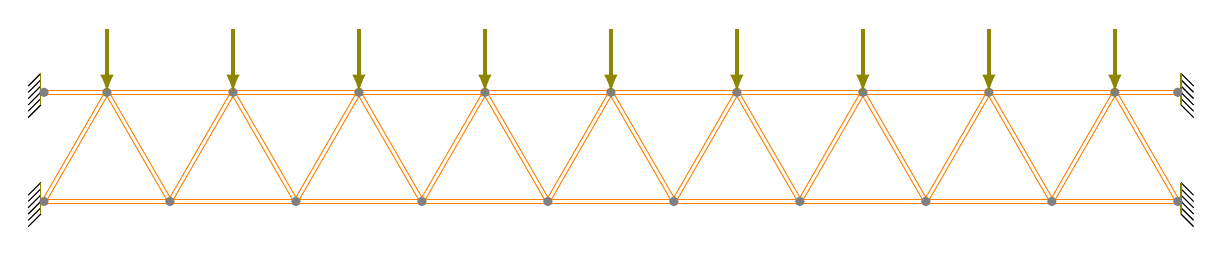
\begin{tikzpicture}[scale=0.8]

\pgfmathsetmacro{\X}{0}
\pgfmathsetmacro{\Y}{0}
\foreach \x in {-0.2,-0.1,...,0.3}{
\draw (\X-0.05,\Y+\x) --++ (-0.2,-0.2);
}
\draw[olive] (\X-0.05,\Y-0.2) - - ++(0,0.5);

\pgfmathsetmacro{\X}{0}
\pgfmathsetmacro{\Y}{1.7320508075688772}
\foreach \x in {-0.2,-0.1,...,0.3}{
\draw (\X-0.05,\Y+\x) --++ (-0.2,-0.2);
}
\draw[olive] (\X-0.05,\Y-0.2) - - ++(0,0.5);

\pgfmathsetmacro{\X}{18}
\pgfmathsetmacro{\Y}{0}
\foreach \x in {-0.2,-0.1,...,0.3}{
\draw (\X+0.05,\Y+\x) --++ (0.2,-0.2);
}
\draw[olive] (\X+0.05,\Y-0.2) - - ++(0,0.5);

\pgfmathsetmacro{\X}{18}
\pgfmathsetmacro{\Y}{1.7320508075688772}
\foreach \x in {-0.2,-0.1,...,0.3}{
\draw (\X+0.05,\Y+\x) --++ (0.2,-0.2);
}
\draw[olive] (\X+0.05,\Y-0.2) - - ++(0,0.5);

\draw[orange, double distance = 1pt] (0,1.7320508075688772) - - (1.0,1.7320508075688772);
\draw[orange, double distance = 1pt] (0.0,0) - - (2.0,0);
\draw[orange, double distance = 1pt] (2.0,0) - - (1.0,1.7320508075688772);
\draw[orange, double distance = 1pt] (1.0,1.7320508075688772) - - (0.0,0);
\draw[orange, double distance = 1pt] (1.0,1.7320508075688772) - - (3.0,1.7320508075688772);
\draw[orange, double distance = 1pt] (2.0,0) - - (4.0,0);
\draw[orange, double distance = 1pt] (4.0,0) - - (3.0,1.7320508075688772);
\draw[orange, double distance = 1pt] (3.0,1.7320508075688772) - - (2.0,0);
\draw[orange, double distance = 1pt] (3.0,1.7320508075688772) - - (5.0,1.7320508075688772);
\draw[orange, double distance = 1pt] (4.0,0) - - (6.0,0);
\draw[orange, double distance = 1pt] (6.0,0) - - (5.0,1.7320508075688772);
\draw[orange, double distance = 1pt] (5.0,1.7320508075688772) - - (4.0,0);
\draw[orange, double distance = 1pt] (5.0,1.7320508075688772) - - (7.0,1.7320508075688772);
\draw[orange, double distance = 1pt] (6.0,0) - - (8.0,0);
\draw[orange, double distance = 1pt] (8.0,0) - - (7.0,1.7320508075688772);
\draw[orange, double distance = 1pt] (7.0,1.7320508075688772) - - (6.0,0);
\draw[orange, double distance = 1pt] (7.0,1.7320508075688772) - - (9.0,1.7320508075688772);
\draw[orange, double distance = 1pt] (8.0,0) - - (10.0,0);
\draw[orange, double distance = 1pt] (10.0,0) - - (9.0,1.7320508075688772);
\draw[orange, double distance = 1pt] (9.0,1.7320508075688772) - - (8.0,0);
\draw[orange, double distance = 1pt] (9.0,1.7320508075688772) - - (11.0,1.7320508075688772);
\draw[orange, double distance = 1pt] (10.0,0) - - (12.0,0);
\draw[orange, double distance = 1pt] (12.0,0) - - (11.0,1.7320508075688772);
\draw[orange, double distance = 1pt] (11.0,1.7320508075688772) - - (10.0,0);
\draw[orange, double distance = 1pt] (11.0,1.7320508075688772) - - (13.0,1.7320508075688772);
\draw[orange, double distance = 1pt] (12.0,0) - - (14.0,0);
\draw[orange, double distance = 1pt] (14.0,0) - - (13.0,1.7320508075688772);
\draw[orange, double distance = 1pt] (13.0,1.7320508075688772) - - (12.0,0);
\draw[orange, double distance = 1pt] (13.0,1.7320508075688772) - - (15.0,1.7320508075688772);
\draw[orange, double distance = 1pt] (14.0,0) - - (16.0,0);
\draw[orange, double distance = 1pt] (16.0,0) - - (15.0,1.7320508075688772);
\draw[orange, double distance = 1pt] (15.0,1.7320508075688772) - - (14.0,0);
\draw[orange, double distance = 1pt] (15.0,1.7320508075688772) - - (17.0,1.7320508075688772);
\draw[orange, double distance = 1pt] (16.0,0) - - (18.0,0);
\draw[orange, double distance = 1pt] (18.0,0) - - (17.0,1.7320508075688772);
\draw[orange, double distance = 1pt] (17.0,1.7320508075688772) - - (16.0,0);
\draw[orange, double distance = 1pt] (17.0,1.7320508075688772) - - (18.0,1.7320508075688772);
\path[fill=black]  (0,1.7320508075688772) circle (.75mm) [fill=gray];
\path[fill=black]  (0.0,0) circle (.75mm) [fill=gray];
\path[fill=black]  (1.0,1.7320508075688772) circle (.75mm) [fill=gray];
\path[fill=black]  (2.0,0) circle (.75mm) [fill=gray];
\path[fill=black]  (3.0,1.7320508075688772) circle (.75mm) [fill=gray];
\path[fill=black]  (4.0,0) circle (.75mm) [fill=gray];
\path[fill=black]  (5.0,1.7320508075688772) circle (.75mm) [fill=gray];
\path[fill=black]  (6.0,0) circle (.75mm) [fill=gray];
\path[fill=black]  (7.0,1.7320508075688772) circle (.75mm) [fill=gray];
\path[fill=black]  (8.0,0) circle (.75mm) [fill=gray];
\path[fill=black]  (9.0,1.7320508075688772) circle (.75mm) [fill=gray];
\path[fill=black]  (10.0,0) circle (.75mm) [fill=gray];
\path[fill=black]  (11.0,1.7320508075688772) circle (.75mm) [fill=gray];
\path[fill=black]  (12.0,0) circle (.75mm) [fill=gray];
\path[fill=black]  (13.0,1.7320508075688772) circle (.75mm) [fill=gray];
\path[fill=black]  (14.0,0) circle (.75mm) [fill=gray];
\path[fill=black]  (15.0,1.7320508075688772) circle (.75mm) [fill=gray];
\path[fill=black]  (16.0,0) circle (.75mm) [fill=gray];
\path[fill=black]  (17.0,1.7320508075688772) circle (.75mm) [fill=gray];
\path[fill=black]  (18.0,0) circle (.75mm) [fill=gray];
\path[fill=black]  (18.0,1.7320508075688772) circle (.75mm) [fill=gray];

\foreach \x in {1,3,...,18}{
\draw[very thick,olive,latex-] (\x,1.7320508075688772)--++(0,1);
}

\end{tikzpicture}
\end{center}

On admet que le système élémentaire d'une barre faisant un angle $\theta$ avec l'horizontal est donnée par:
\[\left(\begin{array}{l} 
F_{1}^x\\F_{1}^y\\F_{2}^x\\F_{2}^y
\end{array}\right)   = \frac{EA}{L}\left(\begin{array}{rrrr} 
C^2&CS&-C^2&-CS\\
CS&S^2&-CS&-S^2\\
-C^2&-CS&C^2&CS\\
-CS&-S^2&CS&S^2
\end{array}\right)\left(\begin{array}{l} 
U_{1}^x\\U_{1}^y\\U_{2}^x\\U_{2}^y
\end{array}\right)  \]
où  $C=\cos\theta$ et $S=\sin\theta$.

%\input{mef3.tex} 
\begin{enumerate}
\item Copier l'annexe A dans votre document Datalore et faire tourner le programme python.
\item Déterminer les réactions des appuis et la flèche maximale.
\end{enumerate}

\subsection*{Poutre en flexion}
\begin{center}
 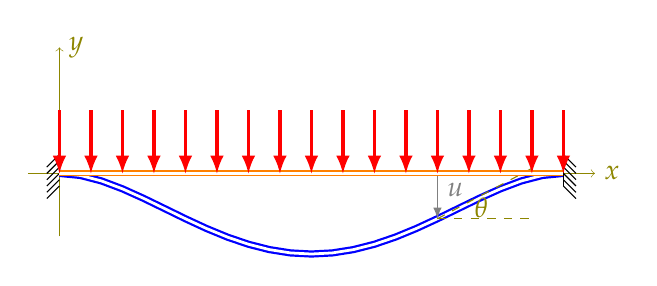
\begin{tikzpicture}[scale=0.8]
\draw  [very thin, olive] [->]  (-0.5,0) -- (8.5,0) node[right] {$x$};
\draw  [very thin, olive] [->]  (0,-1) -- (0,2) node[right] {$y$};
\draw [line width=2mm,blue,thick=6,domain=0:8,double distance = 1pt] plot(\x,{-(\x*\x-8*\x)^2/200});
%\draw  [line width=0.2mm, red] [->]  (8,0.5) -- (8,-1.28);
%\draw[very thick,red,latex-] (8,-1.28)--(8,0.5) node[anchor=east]{$P$};
\draw[gray,latex-] (6,-0.72)--(6,0) node[below right]{$u$};
\draw[olive,dashed] (6,-0.72)--++(1.5,0) ;
\draw[olive,dashed] (6,-0.72)--++(1.5,0.8) ;
\draw[olive] (6.7,-0.55) node{$\theta$};;

\pgfmathsetmacro{\y}{2}
\foreach \x in {-0.2,-0.1,...,0.3}{
\draw (0,\x) --++ (-0.2,-0.2);
\draw[line width=0.2mm,orange, double distance = 1pt] (0,0) - - (8,0);
}

\pgfmathsetmacro{\X}{8}
\foreach \x in {-0.2,-0.1,...,0.3}{
\draw (\X+0,\x) --++ (0.2,-0.2);
}
\draw (\X+0,-0.2) --++ (0,0.5);
\foreach \x in {0,0.5,...,8}{
\draw[very thick,red,latex-] (\x,0)--++(0,1);
}
\end{tikzpicture} 
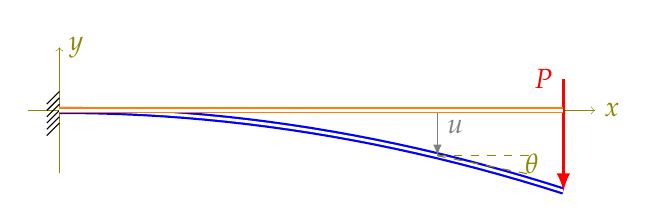
\begin{tikzpicture}[scale=0.8]
\draw  [very thin, olive] [->]  (-0.5,0) -- (8.5,0) node[right] {$x$};
\draw  [very thin, olive] [->]  (0,-1) -- (0,1) node[right] {$y$};
\draw [line width=2mm,blue,thick=6,domain=0:8,double distance = 1pt] plot(\x,{-\x*\x/50});
%\draw  [line width=0.2mm, red] [->]  (8,0.5) -- (8,-1.28);
\draw[very thick,red,latex-] (8,-1.28)--(8,0.5) node[anchor=east]{$P$};
\draw[gray,latex-] (6,-0.72)--(6,0) node[below right]{$u$};
\draw[olive,dashed] (6,-0.72)--++(1.5,0) ;
\draw[olive,dashed] (6,-0.72)--++(1.5,-0.3) ;
\draw[olive] (7.5,-0.85) node{$\theta$};;

\pgfmathsetmacro{\y}{2}
\foreach \x in {-0.2,-0.1,...,0.3}{
\draw (0,\x) --++ (-0.2,-0.2);
}
\draw[line width=0.2mm,orange, double distance = 1pt] (0,0) - - (8,0);
\end{tikzpicture} 

\end{center}

La formulation variationnelle d'une poutre en flexion simple est de la forme (TD3):
\[
({\cal P}_v)\;\left\{
\begin{array}{l}
\mbox{Trouver } u\in V \mbox{ vérifiant}\\
a(u,v)=\ell(v)\quad \forall v\in V
\end{array}
\right.
\]

où \[ a(u,v)=\displaystyle EI_z\int_0^L\frac{\de^2 u}{dx^2}\cdot \frac{\de^2 v}{dx^2}\de x\]
et \[ \ell(v)=\displaystyle \int_0^L p\cdot v(x)\de x+F_0 \cdot v(0)+F_L \cdot v(L)+M_0 \cdot \frac{\partial v}{\partial x}(0)+M_L \cdot \frac{\partial v}{\partial x}(L)\]
On choisit un élément fini de Hermite de type (1) qui utilise les déplacements et leur dérivées comme degrés de liberté. D'où  la matrice élémentaire :
\[\left(\begin{array}{r} 
f_{1}^y\\M_1\\f_{2}^y\\M_2
\end{array}\right)=\frac{EI}{L^3}\left(\begin{array}{rrrr} 
12&6L&-12&6L\\
6L&4L^2&-6L&2L^2\\
-12&-6L&12&-6L\\
6L&2L^2&-6L&4L^2
\end{array}\right) \left(\begin{array}{l} 
u_{1}^y\\\theta_1\\u_{2}^y\\\theta_2
\end{array}\right)
\]

Écrire un programme python permettant de résoudre numériquement l'équation de la poutre en flexion simple par la méthode des éléments finis.

Application numérique:  on donne : $A=r^2$, $I=\frac{1}{12}r^4$, où $r=2\mbox{cm}$ , $L=10 m$ , $E=200$GPa , $p =-200$N.
 
 Exécuter votre programme python dans les deux cas suivants:
 \begin{enumerate}
 \item La poutre est encastrée aux extrémités (déplacement $u$ et angle $\theta$ sont simultanément nuls en $0$ et en $L$).
 \begin{center}
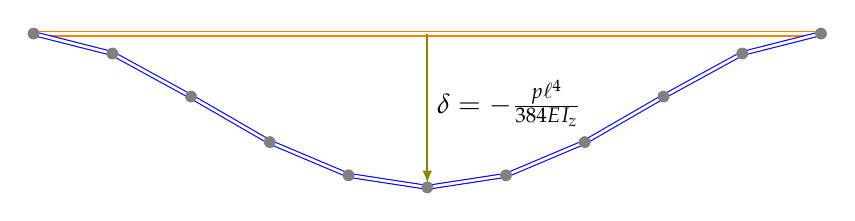
\begin{tikzpicture}[scale=1]
\draw[line width=0.2mm,orange, double distance = 1pt] (0,0) - - (10,0);
\draw[line width=0.2mm,olive,-latex] (5,0) - - (5,-1.9);
\draw(5,-1.3) node[above right]{$\delta=-\frac{p\ell^4}{384EI_z}$};
\draw[blue, double distance = 1pt] (0.0,0.0) - - (1.0,-0.2531249999999979);
\draw[blue, double distance = 1pt] (1.0,-0.2531249999999979) - - (2.0,-0.7999999999999927);
\draw[blue, double distance = 1pt] (2.0,-0.7999999999999927) - - (3.0,-1.3781249999999863);
\draw[blue, double distance = 1pt] (3.0,-1.3781249999999863) - - (4.0,-1.79999999999998);
\draw[blue, double distance = 1pt] (4.0,-1.79999999999998) - - (5.0,-1.953124999999976);
\draw[blue, double distance = 1pt] (5.0,-1.953124999999976) - - (6.0,-1.799999999999976);
\draw[blue, double distance = 1pt] (6.0,-1.799999999999976) - - (7.0,-1.3781249999999807);
\draw[blue, double distance = 1pt] (7.0,-1.3781249999999807) - - (8.0,-0.7999999999999886);
\draw[blue, double distance = 1pt] (8.0,-0.7999999999999886) - - (9.0,-0.2531249999999965);
\draw[blue, double distance = 1pt] (9.0,-0.2531249999999965) - - (10.0,0.0);
\path[fill=black]  (0.0,0.0) circle (.75mm) [fill=gray];
\path[fill=black]  (1.0,-0.2531249999999979) circle (.75mm) [fill=gray];
\path[fill=black]  (2.0,-0.7999999999999927) circle (.75mm) [fill=gray];
\path[fill=black]  (3.0,-1.3781249999999863) circle (.75mm) [fill=gray];
\path[fill=black]  (4.0,-1.79999999999998) circle (.75mm) [fill=gray];
\path[fill=black]  (5.0,-1.953124999999976) circle (.75mm) [fill=gray];
\path[fill=black]  (6.0,-1.799999999999976) circle (.75mm) [fill=gray];
\path[fill=black]  (7.0,-1.3781249999999807) circle (.75mm) [fill=gray];
\path[fill=black]  (8.0,-0.7999999999999886) circle (.75mm) [fill=gray];
\path[fill=black]  (9.0,-0.2531249999999965) circle (.75mm) [fill=gray];
\path[fill=black]  (10.0,0.0) circle (.75mm) [fill=gray];
\end{tikzpicture}
\end{center}
On rappelle (cf TD3)  que le second membre élémentaire d'une poutre soumise uniquement à des charges linéiques de densité $p(x)$ est:
\[\left(\begin{array}{r} 
f_{1}^y\\M_1\\f_{2}^y\\M_2
\end{array}\right)=\left(\begin{array}{r} 
\frac{pL}{2}\\\frac{pL^2}{12}\\\frac{pL}{2}\\-\frac{pL^2}{12}
\end{array}\right)\]
 \item La poutre est encastrée à son origine $0$ (déplacement $u$ et angle $\theta$ sont simultanément nuls). Une force verticale $F=-10N$ est appliquée à l'autre extrémité $L$, avec un moment nul $M_L=0$.
 On rappelle (cf TD3)  que le second membre élémentaire d'une poutre soumise uniquement à une force ponctuelle $F$  en son extrémité $L$  est:
\[\left(\begin{array}{r} 
f_{1}^y\\M_1\\f_{2}^y\\M_2
\end{array}\right)=\left(\begin{array}{r} 
0\\0\\F\\0
\end{array}\right)\]

 

\begin{center}
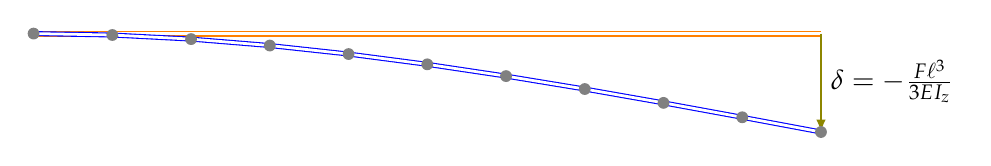
\begin{tikzpicture}[scale=1]
\draw[line width=0.2mm,orange, double distance = 1pt] (0,0) - - (10,0);
\draw[line width=0.2mm,olive,-latex] (10,0) - - (10,-1.25); 
\draw (10,-1) node[above right]{$\delta=-\frac{F\ell^3}{3EI_z}$};
\draw[blue, double distance = 1pt] (0.0,0.0) - - (1.0,-0.01812499999999584);
\draw[blue, double distance = 1pt] (1.0,-0.01812499999999584) - - (2.0,-0.06999999999998444);
\draw[blue, double distance = 1pt] (2.0,-0.06999999999998444) - - (3.0,-0.15187499999996742);
\draw[blue, double distance = 1pt] (3.0,-0.15187499999996742) - - (4.0,-0.2599999999999464);
\draw[blue, double distance = 1pt] (4.0,-0.2599999999999464) - - (5.0,-0.39062499999992295);
\draw[blue, double distance = 1pt] (5.0,-0.39062499999992295) - - (6.0,-0.5399999999998988);
\draw[blue, double distance = 1pt] (6.0,-0.5399999999998988) - - (7.0,-0.7043749999998752);
\draw[blue, double distance = 1pt] (7.0,-0.7043749999998752) - - (8.0,-0.8799999999998527);
\draw[blue, double distance = 1pt] (8.0,-0.8799999999998527) - - (9.0,-1.063124999999831);
\draw[blue, double distance = 1pt] (9.0,-1.063124999999831) - - (10.0,-1.2499999999998095);
\path[fill=black]  (0.0,0.0) circle (.75mm) [fill=gray];
\path[fill=black]  (1.0,-0.01812499999999584) circle (.75mm) [fill=gray];
\path[fill=black]  (2.0,-0.06999999999998444) circle (.75mm) [fill=gray];
\path[fill=black]  (3.0,-0.15187499999996742) circle (.75mm) [fill=gray];
\path[fill=black]  (4.0,-0.2599999999999464) circle (.75mm) [fill=gray];
\path[fill=black]  (5.0,-0.39062499999992295) circle (.75mm) [fill=gray];
\path[fill=black]  (6.0,-0.5399999999998988) circle (.75mm) [fill=gray];
\path[fill=black]  (7.0,-0.7043749999998752) circle (.75mm) [fill=gray];
\path[fill=black]  (8.0,-0.8799999999998527) circle (.75mm) [fill=gray];
\path[fill=black]  (9.0,-1.063124999999831) circle (.75mm) [fill=gray];
\path[fill=black]  (10.0,-1.2499999999998095) circle (.75mm) [fill=gray];
\end{tikzpicture}
\end{center}
\item On reprend la poutre de la question 2 et on ajoute un appui simple au milieu:
\begin{center}
\begin{tikzpicture}[scale=0.8]
\draw  [very thin, olive] [->]  (-0.5,0) -- (8.5,0) node[right] {$x$};
\draw  [very thin, olive] [->]  (0,-1.5) -- (0,3) node[right] {$y$};
%\draw [line width=2mm,blue,thick=6,domain=0:8,double distance = 1pt] plot(\x,{-\x*\x/50});
%\draw  [line width=0.2mm, red] [->]  (8,0.5) -- (8,-1.28);
\draw[very thick,red,latex-] (8,0)--(8,2) node[anchor=east]{$P$};
%\draw[gray,latex-] (6,-0.72)--(6,0) node[below right]{$u$};
\draw[gray,line width=2mm,thick=6] (4,-0.08)--++(0.25,-0.25)--++(-0.5,0)--++(0.25,0.25) ;
\pgfmathsetmacro{\y}{2}
\foreach \x in {3.77,3.87,...,4.27}{
\draw (\x,-0.33) --++ (-0.1,-0.15);
}
%\draw[olive] (7.5,-0.85) node{$\theta$};;

\pgfmathsetmacro{\y}{2}
\foreach \x in {-0.2,-0.1,...,0.3}{
\draw (0,\x) --++ (-0.2,-0.2);
}
\draw[line width=0.2mm,orange, double distance = 1pt] (0,0) - - (8,0);
\end{tikzpicture} 

\end{center}

 \end{enumerate}
Dans les trois cas calculer les flèches maximales, les angles de torsion et les réactions aux points particuliers. Comparer avec les résultats théoriques.
%\input{mef2.tex} 
%%%%%%%%%%%%%%%%%%%%%%%%%%%%%%%%%%%%%%%%%%%%%%%%%%%%%%%%%

  
  
  
  
  %%%%%%%%%%%%%%%%%%%%%%%%%%%%%%%%%%%%%%%%%%%%%%%%%%  
    

    
    \hypertarget{exercice1}{%
\section*{Annexe A: Exercice1}\label{exercice1}}
    \begin{tcolorbox}[breakable, size=fbox, boxrule=1pt, pad at break*=1mm,colback=cellbackground, colframe=cellborder]
\prompt{In}{incolor}{1}{\boxspacing}
\begin{Verbatim}[commandchars=\\\{\}]
\PY{k+kn}{import} \PY{n+nn}{numpy} \PY{k}{as} \PY{n+nn}{np}
\PY{k+kn}{import} \PY{n+nn}{math}
\PY{k+kn}{import} \PY{n+nn}{matplotlib}\PY{n+nn}{.}\PY{n+nn}{pyplot} \PY{k}{as} \PY{n+nn}{plt}
\end{Verbatim}
\end{tcolorbox}

    \hypertarget{donnuxe9es-et-constantes-physiques}{%
\subsubsection*{Données et constantes
physiques}\label{donnuxe9es-et-constantes-physiques}}

\begin{itemize}
\tightlist
\item
  Le pont est de longueur \(L=10\) m.
\item
  Le nombre des sommets sur la partie inférieur du pont est \(N+1=11\).
\item
  Les poutres ont une même longueur: \(h=1\)m, et une même section
  rectangulaire 10 mm \(\times\) 20 mm, soit
  \(A=200\times 10^{-6}\mbox{ m}^2\).
\item
  On applique en chaque noeud du tablier une charge \(P=-3000\) N.
\item
  Le module de Young est \(E=200000\) MPa.
\end{itemize}

    \begin{tcolorbox}[breakable, size=fbox, boxrule=1pt, pad at break*=1mm,colback=cellbackground, colframe=cellborder]
\prompt{In}{incolor}{2}{\boxspacing}
\begin{Verbatim}[commandchars=\\\{\}]
\PY{n}{L} \PY{o}{=} \PY{l+m+mf}{10.}
\PY{n}{A} \PY{o}{=} \PY{l+m+mi}{200} \PY{o}{*} \PY{l+m+mf}{1E\PYZhy{}6}
\PY{n}{E} \PY{o}{=} \PY{l+m+mi}{200} \PY{o}{*} \PY{l+m+mf}{1E9}
\PY{n}{P} \PY{o}{=} \PY{l+m+mi}{30000} \PY{c+c1}{\PYZsh{}50000}
\PY{n}{N}\PY{o}{=}\PY{l+m+mi}{10} \PY{c+c1}{\PYZsh{} Nombre des poutres sur la partie inférieur du pont.}
\PY{n}{h}\PY{o}{=}\PY{n}{L}\PY{o}{/}\PY{n}{N}    \PY{c+c1}{\PYZsh{} longueur élémentaire}
\end{Verbatim}
\end{tcolorbox}

    On pose \(r_3=\sqrt 3\)

    \begin{tcolorbox}[breakable, size=fbox, boxrule=1pt, pad at break*=1mm,colback=cellbackground, colframe=cellborder]
\prompt{In}{incolor}{3}{\boxspacing}
\begin{Verbatim}[commandchars=\\\{\}]
\PY{n}{r3}\PY{o}{=}\PY{n}{math}\PY{o}{.}\PY{n}{sqrt}\PY{p}{(}\PY{l+m+mi}{3}\PY{p}{)}
\end{Verbatim}
\end{tcolorbox}

    \hypertarget{guxe9omuxe9trie-du-probluxe8me}{%
\subsection*{Géométrie du
problème}\label{guxe9omuxe9trie-du-probluxe8me}}

\hypertarget{maillage-les-uxe9luxe9ments-finis-sont-les-poutres}{%
\subsubsection*{Maillage: les éléments finis sont les
poutres}\label{maillage-les-uxe9luxe9ments-finis-sont-les-poutres}}

    \begin{tcolorbox}[breakable, size=fbox, boxrule=1pt, pad at break*=1mm,colback=cellbackground, colframe=cellborder]
\prompt{In}{incolor}{4}{\boxspacing}
\begin{Verbatim}[commandchars=\\\{\}]
\PY{n}{Points}\PY{o}{=}\PY{p}{[}\PY{p}{]}  \PY{c+c1}{\PYZsh{} Liste des sommets}
\PY{n}{Points}\PY{o}{.}\PY{n}{append}\PY{p}{(}\PY{p}{[}\PY{o}{\PYZhy{}}\PY{n}{h}\PY{o}{/}\PY{l+m+mi}{2}\PY{p}{,}\PY{n}{r3}\PY{o}{*}\PY{n}{h}\PY{o}{/}\PY{l+m+mi}{2}\PY{p}{]}\PY{p}{)}
\PY{k}{for} \PY{n}{i} \PY{o+ow}{in} \PY{n+nb}{range}\PY{p}{(}\PY{n}{N}\PY{p}{)}\PY{p}{:}
    \PY{n}{Points}\PY{o}{.}\PY{n}{append}\PY{p}{(}\PY{p}{[}\PY{n}{i}\PY{o}{*}\PY{n}{h}\PY{p}{,}\PY{l+m+mi}{0}\PY{p}{]}\PY{p}{)}
    \PY{n}{Points}\PY{o}{.}\PY{n}{append}\PY{p}{(}\PY{p}{[}\PY{n}{i}\PY{o}{*}\PY{n}{h}\PY{o}{+}\PY{n}{h}\PY{o}{/}\PY{l+m+mi}{2}\PY{p}{,} \PY{n}{r3}\PY{o}{*}\PY{n}{h}\PY{o}{/}\PY{l+m+mi}{2}\PY{p}{]}\PY{p}{)}
\PY{n}{Points}\PY{o}{.}\PY{n}{append}\PY{p}{(}\PY{p}{[}\PY{n}{N}\PY{o}{*}\PY{n}{h}\PY{p}{,} \PY{l+m+mi}{0}\PY{p}{]}\PY{p}{)}
\PY{n}{Points}\PY{o}{.}\PY{n}{append}\PY{p}{(}\PY{p}{[}\PY{n}{N}\PY{o}{*}\PY{n}{h}\PY{o}{+}\PY{n}{h}\PY{o}{/}\PY{l+m+mi}{2}\PY{p}{,} \PY{n}{r3} \PY{o}{*} \PY{n}{h}\PY{o}{/}\PY{l+m+mi}{2}\PY{p}{]}\PY{p}{)}
\end{Verbatim}
\end{tcolorbox}

    \begin{tcolorbox}[breakable, size=fbox, boxrule=1pt, pad at break*=1mm,colback=cellbackground, colframe=cellborder]
\prompt{In}{incolor}{5}{\boxspacing}
\begin{Verbatim}[commandchars=\\\{\}]
\PY{n}{Barres}\PY{o}{=}\PY{p}{[}\PY{p}{]}  \PY{c+c1}{\PYZsh{} Table de connectivité}
\PY{k}{for} \PY{n}{k} \PY{o+ow}{in} \PY{n+nb}{range}\PY{p}{(}\PY{n}{N}\PY{p}{)}\PY{p}{:}
    \PY{n}{Barres}\PY{o}{.}\PY{n}{append}\PY{p}{(}\PY{p}{[}\PY{l+m+mi}{2} \PY{o}{*} \PY{n}{k} \PY{p}{,} \PY{l+m+mi}{2} \PY{o}{*} \PY{n}{k} \PY{o}{+} \PY{l+m+mi}{2}\PY{p}{]}\PY{p}{)} \PY{c+c1}{\PYZsh{} poutres horizontales supérieures}
    \PY{n}{Barres}\PY{o}{.}\PY{n}{append}\PY{p}{(}\PY{p}{[}\PY{l+m+mi}{2}\PY{o}{*}\PY{n}{k}\PY{o}{+}\PY{l+m+mi}{1}\PY{p}{,}\PY{l+m+mi}{2}\PY{o}{*}\PY{n}{k}\PY{o}{+}\PY{l+m+mi}{3}\PY{p}{]}\PY{p}{)} \PY{c+c1}{\PYZsh{} poutres horizontales inférieures}
    \PY{n}{Barres}\PY{o}{.}\PY{n}{append}\PY{p}{(}\PY{p}{[}\PY{l+m+mi}{2} \PY{o}{*} \PY{n}{k} \PY{o}{+} \PY{l+m+mi}{1}\PY{p}{,} \PY{l+m+mi}{2} \PY{o}{*} \PY{n}{k} \PY{o}{+} \PY{l+m+mi}{2}\PY{p}{]}\PY{p}{)} \PY{c+c1}{\PYZsh{} poutres obliques /}
    \PY{n}{Barres}\PY{o}{.}\PY{n}{append}\PY{p}{(}\PY{p}{[} \PY{l+m+mi}{2} \PY{o}{*} \PY{n}{k}\PY{o}{+}\PY{l+m+mi}{2}\PY{p}{,} \PY{l+m+mi}{2} \PY{o}{*} \PY{n}{k} \PY{o}{+}\PY{l+m+mi}{3} \PY{p}{]}\PY{p}{)} \PY{c+c1}{\PYZsh{} poutres obliques \PYZbs{}}
    

\PY{n}{Barres}\PY{o}{.}\PY{n}{append}\PY{p}{(}\PY{p}{[}\PY{l+m+mi}{2}\PY{o}{*}\PY{n}{N}\PY{p}{,}\PY{l+m+mi}{2}\PY{o}{*}\PY{n}{N}\PY{o}{+}\PY{l+m+mi}{2}\PY{p}{]}\PY{p}{)} \PY{c+c1}{\PYZsh{} la dernière poutre horizontale supérieure}
\end{Verbatim}
\end{tcolorbox}

    \begin{tcolorbox}[breakable, size=fbox, boxrule=1pt, pad at break*=1mm,colback=cellbackground, colframe=cellborder]
\prompt{In}{incolor}{6}{\boxspacing}
\begin{Verbatim}[commandchars=\\\{\}]
\PY{k}{def} \PY{n+nf}{cotes}\PY{p}{(}\PY{p}{)}\PY{p}{:}
    \PY{n}{plt}\PY{o}{.}\PY{n}{plot}\PY{p}{(}\PY{p}{[}\PY{l+m+mi}{0}\PY{p}{,} \PY{o}{\PYZhy{}}\PY{n}{h}\PY{o}{/}\PY{l+m+mi}{2}\PY{p}{,}\PY{o}{\PYZhy{}}\PY{n}{h}\PY{o}{/}\PY{l+m+mi}{2}\PY{p}{,}\PY{l+m+mi}{0}\PY{p}{,}\PY{l+m+mi}{0}\PY{p}{]}\PY{p}{,} \PY{p}{[}\PY{l+m+mi}{0}\PY{p}{,} \PY{n}{r3}\PY{o}{*}\PY{n}{h}\PY{o}{/}\PY{l+m+mi}{2}\PY{p}{,}\PY{o}{\PYZhy{}}\PY{l+m+mi}{3}\PY{p}{,}\PY{o}{\PYZhy{}}\PY{l+m+mi}{3}\PY{p}{,}\PY{l+m+mi}{0}\PY{p}{]}\PY{p}{,} \PY{n}{color}\PY{o}{=}\PY{l+s+s1}{\PYZsq{}}\PY{l+s+s1}{green}\PY{l+s+s1}{\PYZsq{}}\PY{p}{,} \PY{n}{linestyle}\PY{o}{=}\PY{l+s+s1}{\PYZsq{}}\PY{l+s+s1}{solid}\PY{l+s+s1}{\PYZsq{}}\PY{p}{)}
    \PY{n}{plt}\PY{o}{.}\PY{n}{plot}\PY{p}{(}\PY{p}{[}\PY{n}{L}\PY{p}{,} \PY{n}{L}\PY{o}{+}\PY{n}{h}\PY{o}{/}\PY{l+m+mi}{2}\PY{p}{,}\PY{n}{L}\PY{o}{+}\PY{n}{h}\PY{o}{/}\PY{l+m+mi}{2}\PY{p}{,}\PY{n}{L}\PY{p}{,}\PY{n}{L}\PY{p}{]}\PY{p}{,} \PY{p}{[}\PY{l+m+mi}{0}\PY{p}{,} \PY{n}{r3}\PY{o}{*}\PY{n}{h}\PY{o}{/}\PY{l+m+mi}{2}\PY{p}{,}\PY{o}{\PYZhy{}}\PY{l+m+mi}{3}\PY{p}{,}\PY{o}{\PYZhy{}}\PY{l+m+mi}{3}\PY{p}{,}\PY{l+m+mi}{0}\PY{p}{]}\PY{p}{,} \PY{n}{color}\PY{o}{=}\PY{l+s+s1}{\PYZsq{}}\PY{l+s+s1}{green}\PY{l+s+s1}{\PYZsq{}}\PY{p}{,} \PY{n}{linestyle}\PY{o}{=}\PY{l+s+s1}{\PYZsq{}}\PY{l+s+s1}{solid}\PY{l+s+s1}{\PYZsq{}}\PY{p}{)}
\end{Verbatim}
\end{tcolorbox}

    \begin{tcolorbox}[breakable, size=fbox, boxrule=1pt, pad at break*=1mm,colback=cellbackground, colframe=cellborder]
\prompt{In}{incolor}{7}{\boxspacing}
\begin{Verbatim}[commandchars=\\\{\}]
\PY{n}{cotes}\PY{p}{(}\PY{p}{)}
\PY{k}{for} \PY{n}{p1}\PY{p}{,} \PY{n}{p2} \PY{o+ow}{in} \PY{n}{Barres}\PY{p}{:}
    \PY{n}{x1}\PY{p}{,}\PY{n}{y1} \PY{o}{=} \PY{n}{Points}\PY{p}{[}\PY{n}{p1}\PY{p}{]}
    \PY{n}{x2}\PY{p}{,}\PY{n}{y2} \PY{o}{=} \PY{n}{Points}\PY{p}{[}\PY{n}{p2}\PY{p}{]}
    \PY{n}{plt}\PY{o}{.}\PY{n}{plot}\PY{p}{(}\PY{p}{[}\PY{n}{x1}\PY{p}{,} \PY{n}{x2}\PY{p}{]}\PY{p}{,} \PY{p}{[}\PY{n}{y1}\PY{p}{,} \PY{n}{y2}\PY{p}{]}\PY{p}{,} \PY{n}{color}\PY{o}{=}\PY{l+s+s1}{\PYZsq{}}\PY{l+s+s1}{red}\PY{l+s+s1}{\PYZsq{}}\PY{p}{,} \PY{n}{linestyle}\PY{o}{=}\PY{l+s+s1}{\PYZsq{}}\PY{l+s+s1}{solid}\PY{l+s+s1}{\PYZsq{}}\PY{p}{)}
    \PY{n}{plt}\PY{o}{.}\PY{n}{axis}\PY{p}{(}\PY{l+s+s1}{\PYZsq{}}\PY{l+s+s1}{equal}\PY{l+s+s1}{\PYZsq{}}\PY{p}{)}   \PY{c+c1}{\PYZsh{} repère orthonormé}
\end{Verbatim}
\end{tcolorbox}

    \begin{center}
    \adjustimage{max size={0.9\linewidth}{0.9\paperheight}}{output_11_0.png}
    \end{center}
    { \hspace*{\fill} \\}
    
    \hypertarget{charges-externes}{%
\subsection*{Charges externes}\label{charges-externes}}

La charge appliquée en un noeud est un triplet:
\([n^{(i)},F^{(i)}_x,F^{(i)}_y]\) 
\begin{itemize}
\item  \(n_i\) est le numéro du nœud
\(i\). 
\item  \(F^{(i)}_x\) est la composante horizontale de la force
appliquée au noeud \(i\). 
\item \(F^{(i)}_y\) est la composante verticale de
la force appliquée au noeud \(i\).
\end{itemize}
    \begin{tcolorbox}[breakable, size=fbox, boxrule=1pt, pad at break*=1mm,colback=cellbackground, colframe=cellborder]
\prompt{In}{incolor}{8}{\boxspacing}
\begin{Verbatim}[commandchars=\\\{\}]
\PY{n}{n} \PY{o}{=} \PY{n+nb}{len}\PY{p}{(}\PY{n}{Points}\PY{p}{)} \PY{o}{*} \PY{l+m+mi}{2}
\PY{c+c1}{\PYZsh{} Liste des charges externes}
\PY{n}{Charges} \PY{o}{=}\PY{p}{[}\PY{p}{[}\PY{l+m+mi}{2}\PY{o}{*}\PY{n}{i}\PY{p}{,}\PY{l+m+mi}{0}\PY{p}{,}\PY{o}{\PYZhy{}}\PY{n}{P}\PY{p}{]} \PY{k}{for} \PY{n}{i} \PY{o+ow}{in} \PY{n+nb}{range}\PY{p}{(}\PY{l+m+mi}{1}\PY{p}{,}\PY{n}{N}\PY{p}{)}\PY{p}{]} 
\PY{c+c1}{\PYZsh{}print(Charges)}
\PY{n}{l} \PY{o}{=} \PY{p}{[}\PY{p}{]} \PY{c+c1}{\PYZsh{} Liste des indices où les déplacements nuls sont appliquées}
\PY{n}{B} \PY{o}{=} \PY{n}{np}\PY{o}{.}\PY{n}{zeros}\PY{p}{(}\PY{n}{n}\PY{p}{,} \PY{n}{dtype}\PY{o}{=}\PY{n+nb}{float}\PY{p}{)}
\PY{k}{for} \PY{n}{q}\PY{p}{,} \PY{n}{a}\PY{p}{,} \PY{n}{b} \PY{o+ow}{in} \PY{n}{Charges}\PY{p}{:}
    \PY{n}{B}\PY{p}{[}\PY{l+m+mi}{2} \PY{o}{*} \PY{n}{q}\PY{p}{]} \PY{o}{=} \PY{n}{a}
    \PY{n}{B}\PY{p}{[}\PY{l+m+mi}{2} \PY{o}{*} \PY{n}{q} \PY{o}{+} \PY{l+m+mi}{1}\PY{p}{]} \PY{o}{=} \PY{n}{b}
\PY{c+c1}{\PYZsh{}print(B)}
\end{Verbatim}
\end{tcolorbox}

    \hypertarget{conditions-aux-appuis}{%
\subsection*{Conditions aux appuis :}\label{conditions-aux-appuis}}

Une condition d'appui est un triplet:
\([n^{(i)},\varepsilon_x,\varepsilon_y]\) 
\begin{itemize}
\item \(n_i\) est le numéro du
noeud \(i\). 
\item \(\varepsilon_x=0\) si le déplacement suivant \(x\) est
bloqué sinon \(\varepsilon_x=1\). 
\item \(\varepsilon_y=0\) si le
déplacement suivant \(y\) est bloqué sinon \(\varepsilon_y=1\).
\end{itemize}


    \begin{tcolorbox}[breakable, size=fbox, boxrule=1pt, pad at break*=1mm,colback=cellbackground, colframe=cellborder]
\prompt{In}{incolor}{9}{\boxspacing}
\begin{Verbatim}[commandchars=\\\{\}]
\PY{n}{Conditions}\PY{o}{=}\PY{p}{[}\PY{p}{[}\PY{l+m+mi}{0}\PY{p}{,}\PY{l+m+mi}{0}\PY{p}{,}\PY{l+m+mi}{0}\PY{p}{]}\PY{p}{,}\PY{p}{[}\PY{l+m+mi}{1}\PY{p}{,}\PY{l+m+mi}{0}\PY{p}{,}\PY{l+m+mi}{0}\PY{p}{]}\PY{p}{,}\PY{p}{[}\PY{l+m+mi}{2}\PY{o}{*}\PY{n}{N}\PY{o}{+}\PY{l+m+mi}{1}\PY{p}{,}\PY{l+m+mi}{0}\PY{p}{,}\PY{l+m+mi}{0}\PY{p}{]}\PY{p}{,}\PY{p}{[}\PY{l+m+mi}{2}\PY{o}{*}\PY{n}{N}\PY{o}{+}\PY{l+m+mi}{2}\PY{p}{,}\PY{l+m+mi}{0}\PY{p}{,}\PY{l+m+mi}{0}\PY{p}{]}\PY{p}{]}
\PY{n}{l} \PY{o}{=} \PY{p}{[}\PY{p}{]} \PY{c+c1}{\PYZsh{} Liste des indices où les déplacements nuls sont appliquées}
\PY{k}{for} \PY{n}{q}\PY{p}{,} \PY{n}{a}\PY{p}{,} \PY{n}{b} \PY{o+ow}{in} \PY{n}{Conditions}\PY{p}{:}
    \PY{k}{if} \PY{n}{a} \PY{o}{==} \PY{l+m+mi}{0}\PY{p}{:}
        \PY{n}{l}\PY{o}{.}\PY{n}{append}\PY{p}{(}\PY{l+m+mi}{2} \PY{o}{*} \PY{n}{q}\PY{p}{)}
    \PY{k}{if} \PY{n}{b} \PY{o}{==} \PY{l+m+mi}{0}\PY{p}{:}
        \PY{n}{l}\PY{o}{.}\PY{n}{append}\PY{p}{(}\PY{l+m+mi}{2} \PY{o}{*} \PY{n}{q} \PY{o}{+} \PY{l+m+mi}{1}\PY{p}{)}
\end{Verbatim}
\end{tcolorbox}

    \hypertarget{matrice-uxe9luxe9mentaire-et-matrice-globale}{%
\subsection*{Matrice élémentaire et matrice
globale}\label{matrice-uxe9luxe9mentaire-et-matrice-globale}}

    \begin{tcolorbox}[breakable, size=fbox, boxrule=1pt, pad at break*=1mm,colback=cellbackground, colframe=cellborder]
\prompt{In}{incolor}{10}{\boxspacing}
\begin{Verbatim}[commandchars=\\\{\}]
\PY{c+c1}{\PYZsh{} Matrice globale}
\PY{n}{M} \PY{o}{=} \PY{n}{np}\PY{o}{.}\PY{n}{zeros}\PY{p}{(}\PY{p}{(}\PY{n}{n}\PY{p}{,} \PY{n}{n}\PY{p}{)}\PY{p}{,} \PY{n}{dtype}\PY{o}{=}\PY{n+nb}{float}\PY{p}{)}
\PY{k}{for} \PY{n}{p1}\PY{p}{,} \PY{n}{p2} \PY{o+ow}{in} \PY{n}{Barres}\PY{p}{:}
    \PY{n}{x1}\PY{p}{,}\PY{n}{y1} \PY{o}{=} \PY{n}{Points}\PY{p}{[}\PY{n}{p1}\PY{p}{]}
    \PY{n}{x2}\PY{p}{,}\PY{n}{y2} \PY{o}{=} \PY{n}{Points}\PY{p}{[}\PY{n}{p2}\PY{p}{]}
    \PY{c+c1}{\PYZsh{}print(\PYZdq{}(\PYZdq{}, x1, \PYZdq{},\PYZdq{}, y1, \PYZdq{}) (\PYZdq{}, x2, \PYZdq{},\PYZdq{}, y2, \PYZdq{})\PYZdq{})}
    \PY{n}{ell} \PY{o}{=} \PY{n}{math}\PY{o}{.}\PY{n}{sqrt}\PY{p}{(}\PY{p}{(}\PY{n}{x2} \PY{o}{\PYZhy{}} \PY{n}{x1}\PY{p}{)} \PY{o}{*}\PY{o}{*} \PY{l+m+mi}{2} \PY{o}{+} \PY{p}{(}\PY{n}{y2} \PY{o}{\PYZhy{}} \PY{n}{y1}\PY{p}{)} \PY{o}{*}\PY{o}{*} \PY{l+m+mi}{2}\PY{p}{)}
    \PY{n}{c} \PY{o}{=} \PY{p}{(}\PY{n}{x2} \PY{o}{\PYZhy{}} \PY{n}{x1}\PY{p}{)} \PY{o}{/} \PY{n}{ell}
    \PY{n}{s} \PY{o}{=} \PY{p}{(}\PY{n}{y2} \PY{o}{\PYZhy{}} \PY{n}{y1}\PY{p}{)} \PY{o}{/} \PY{n}{ell}
    \PY{n}{CS} \PY{o}{=} \PY{n}{np}\PY{o}{.}\PY{n}{mat}\PY{p}{(}\PY{p}{[}\PY{n}{c}\PY{p}{,} \PY{n}{s}\PY{p}{,} \PY{o}{\PYZhy{}}\PY{n}{c}\PY{p}{,} \PY{o}{\PYZhy{}}\PY{n}{s}\PY{p}{]}\PY{p}{,} \PY{n}{dtype}\PY{o}{=}\PY{n+nb}{float}\PY{p}{)}
    \PY{n}{CSt} \PY{o}{=} \PY{n}{np}\PY{o}{.}\PY{n}{transpose}\PY{p}{(}\PY{n}{CS}\PY{p}{)}
    \PY{n}{m} \PY{o}{=} \PY{n}{np}\PY{o}{.}\PY{n}{dot}\PY{p}{(}\PY{n}{CSt}\PY{p}{,} \PY{n}{CS}\PY{p}{)}\PY{o}{*}\PY{n}{A}\PY{o}{*}\PY{n}{E}\PY{o}{/}\PY{n}{ell}
    \PY{c+c1}{\PYZsh{} Assemblage de la matrice globale}
    \PY{k}{for} \PY{n}{r} \PY{o+ow}{in} \PY{n+nb}{range}\PY{p}{(}\PY{l+m+mi}{2}\PY{p}{)}\PY{p}{:}
        \PY{k}{for} \PY{n}{s} \PY{o+ow}{in} \PY{n+nb}{range}\PY{p}{(}\PY{l+m+mi}{2}\PY{p}{)}\PY{p}{:}
            \PY{n}{M}\PY{p}{[}\PY{l+m+mi}{2} \PY{o}{*} \PY{n}{p1}\PY{o}{+}\PY{n}{r}\PY{p}{,} \PY{l+m+mi}{2} \PY{o}{*} \PY{n}{p1}\PY{o}{+}\PY{n}{s}\PY{p}{]} \PY{o}{+}\PY{o}{=} \PY{n}{m}\PY{p}{[}\PY{l+m+mi}{0}\PY{o}{+}\PY{n}{r}\PY{p}{,} \PY{l+m+mi}{0}\PY{o}{+}\PY{n}{s}\PY{p}{]}
            \PY{n}{M}\PY{p}{[}\PY{l+m+mi}{2} \PY{o}{*} \PY{n}{p1} \PY{o}{+} \PY{n}{r}\PY{p}{,} \PY{l+m+mi}{2} \PY{o}{*} \PY{n}{p2} \PY{o}{+} \PY{n}{s}\PY{p}{]} \PY{o}{+}\PY{o}{=} \PY{n}{m}\PY{p}{[}\PY{l+m+mi}{0} \PY{o}{+} \PY{n}{r}\PY{p}{,} \PY{l+m+mi}{2} \PY{o}{+} \PY{n}{s}\PY{p}{]}
            \PY{n}{M}\PY{p}{[}\PY{l+m+mi}{2} \PY{o}{*} \PY{n}{p2} \PY{o}{+} \PY{n}{r}\PY{p}{,} \PY{l+m+mi}{2} \PY{o}{*} \PY{n}{p1} \PY{o}{+} \PY{n}{s}\PY{p}{]} \PY{o}{+}\PY{o}{=} \PY{n}{m}\PY{p}{[}\PY{l+m+mi}{2} \PY{o}{+} \PY{n}{r}\PY{p}{,} \PY{l+m+mi}{0} \PY{o}{+} \PY{n}{s}\PY{p}{]}
            \PY{n}{M}\PY{p}{[}\PY{l+m+mi}{2} \PY{o}{*} \PY{n}{p2} \PY{o}{+} \PY{n}{r}\PY{p}{,} \PY{l+m+mi}{2} \PY{o}{*} \PY{n}{p2} \PY{o}{+} \PY{n}{s}\PY{p}{]} \PY{o}{+}\PY{o}{=} \PY{n}{m}\PY{p}{[}\PY{l+m+mi}{2} \PY{o}{+} \PY{n}{r}\PY{p}{,} \PY{l+m+mi}{2} \PY{o}{+} \PY{n}{s}\PY{p}{]}
\end{Verbatim}
\end{tcolorbox}

    \hypertarget{simplification-du-systuxe8me-linuxe9aire-uxe9limination-des-duxe9placements-connus}{%
\subsection*{Simplification du système linéaire: élimination des
déplacements
connus}\label{simplification-du-systuxe8me-linuxe9aire-uxe9limination-des-duxe9placements-connus}}

    \begin{tcolorbox}[breakable, size=fbox, boxrule=1pt, pad at break*=1mm,colback=cellbackground, colframe=cellborder]
\prompt{In}{incolor}{11}{\boxspacing}
\begin{Verbatim}[commandchars=\\\{\}]
\PY{c+c1}{\PYZsh{} L\PYZsq{}etat initial de la matrice M est conservé dans M0}
\PY{n}{M0} \PY{o}{=} \PY{n}{M}\PY{o}{.}\PY{n}{copy}\PY{p}{(}\PY{p}{)}
\PY{c+c1}{\PYZsh{} Suppression des lignes et colonnes correspondant aux indices des contraintes nulles}
\PY{n}{l}\PY{o}{.}\PY{n}{sort}\PY{p}{(}\PY{p}{)}
\PY{n}{l}\PY{o}{.}\PY{n}{reverse}\PY{p}{(}\PY{p}{)}
\PY{k}{for} \PY{n}{i} \PY{o+ow}{in} \PY{n}{l}\PY{p}{:}
    \PY{n}{M} \PY{o}{=} \PY{n}{np}\PY{o}{.}\PY{n}{delete}\PY{p}{(}\PY{n}{M}\PY{p}{,} \PY{n}{i}\PY{p}{,} \PY{n}{axis}\PY{o}{=}\PY{l+m+mi}{0}\PY{p}{)}
    \PY{n}{M} \PY{o}{=} \PY{n}{np}\PY{o}{.}\PY{n}{delete}\PY{p}{(}\PY{n}{M}\PY{p}{,} \PY{n}{i}\PY{p}{,} \PY{n}{axis}\PY{o}{=}\PY{l+m+mi}{1}\PY{p}{)}
    \PY{n}{B} \PY{o}{=} \PY{n}{np}\PY{o}{.}\PY{n}{delete}\PY{p}{(}\PY{n}{B}\PY{p}{,} \PY{n}{i}\PY{p}{)}
\end{Verbatim}
\end{tcolorbox}

    \hypertarget{ruxe9solution-du-systuxe8me-linuxe9aire}{%
\subsection*{Résolution du système
linéaire}\label{ruxe9solution-du-systuxe8me-linuxe9aire}}

    \begin{tcolorbox}[breakable, size=fbox, boxrule=1pt, pad at break*=1mm,colback=cellbackground, colframe=cellborder]
\prompt{In}{incolor}{12}{\boxspacing}
\begin{Verbatim}[commandchars=\\\{\}]
\PY{c+c1}{\PYZsh{} Inversion du système linéaire}

\PY{n}{deplacement} \PY{o}{=} \PY{n}{np}\PY{o}{.}\PY{n}{linalg}\PY{o}{.}\PY{n}{solve}\PY{p}{(}\PY{n}{M}\PY{p}{,} \PY{n}{B}\PY{p}{)}
\end{Verbatim}
\end{tcolorbox}

    \hypertarget{repruxe9sentation-graphique-de-la-solution}{%
\subsection*{Représentation graphique de la
solution}\label{repruxe9sentation-graphique-de-la-solution}}

    \begin{tcolorbox}[breakable, size=fbox, boxrule=1pt, pad at break*=1mm,colback=cellbackground, colframe=cellborder]
\prompt{In}{incolor}{13}{\boxspacing}
\begin{Verbatim}[commandchars=\\\{\}]
\PY{c+c1}{\PYZsh{} Rétablire les déplacements nuls}
\PY{n}{l}\PY{o}{.}\PY{n}{sort}\PY{p}{(}\PY{p}{)}
\PY{k}{for} \PY{n}{i} \PY{o+ow}{in} \PY{n}{l}\PY{p}{:}
    \PY{n}{deplacement} \PY{o}{=}\PY{n}{np}\PY{o}{.}\PY{n}{insert}\PY{p}{(}\PY{n}{deplacement}\PY{p}{,}\PY{n}{i}\PY{p}{,}\PY{l+m+mi}{0}\PY{p}{)}

\PY{c+c1}{\PYZsh{} Calcul des réactions aux appuis}
\PY{n}{reactions} \PY{o}{=} \PY{n}{M0}\PY{o}{.}\PY{n}{dot}\PY{p}{(}\PY{n}{deplacement}\PY{p}{)}
\PY{c+c1}{\PYZsh{}print(100*\PYZdq{}F\PYZdq{},\PYZdq{}\PYZbs{}n\PYZdq{},reactions,\PYZdq{}\PYZbs{}n\PYZdq{},100*\PYZdq{}F\PYZdq{},\PYZdq{}\PYZbs{}n\PYZdq{})}
\PY{c+c1}{\PYZsh{}print(100*\PYZdq{}?\PYZdq{},\PYZdq{}\PYZbs{}n\PYZdq{},deplacement,\PYZdq{}\PYZbs{}n\PYZdq{},100*\PYZdq{}?\PYZdq{},\PYZdq{}\PYZbs{}n\PYZdq{})}
\PY{c+c1}{\PYZsh{} Pour des raisons graphiques on amplifie delta 10 fois}
\PY{n}{delta}\PY{o}{=}\PY{n}{deplacement}\PY{o}{*}\PY{l+m+mi}{10}
\PY{n}{n}\PY{o}{=}\PY{n+nb}{len}\PY{p}{(}\PY{n}{Points}\PY{p}{)}
\PY{n}{PointsPrim}\PY{o}{=}\PY{p}{[}\PY{p}{]} \PY{c+c1}{\PYZsh{} Position des noeuds après la déformation}
\PY{k}{for} \PY{n}{k} \PY{o+ow}{in} \PY{n+nb}{range}\PY{p}{(}\PY{n}{n}\PY{p}{)}\PY{p}{:}
    \PY{n}{PointsPrim}\PY{o}{.}\PY{n}{append}\PY{p}{(}\PY{p}{[}\PY{n}{delta}\PY{p}{[}\PY{l+m+mi}{2}\PY{o}{*}\PY{n}{k}\PY{p}{]}\PY{o}{+}\PY{n}{Points}\PY{p}{[}\PY{n}{k}\PY{p}{]}\PY{p}{[}\PY{l+m+mi}{0}\PY{p}{]}\PY{p}{,}\PY{n}{delta}\PY{p}{[}\PY{l+m+mi}{2}\PY{o}{*}\PY{n}{k}\PY{o}{+}\PY{l+m+mi}{1}\PY{p}{]}\PY{o}{+}\PY{n}{Points}\PY{p}{[}\PY{n}{k}\PY{p}{]}\PY{p}{[}\PY{l+m+mi}{1}\PY{p}{]}\PY{p}{]}\PY{p}{)}

\PY{k}{for} \PY{p}{[}\PY{n}{p1}\PY{p}{,}\PY{n}{p2}\PY{p}{]} \PY{o+ow}{in} \PY{n}{Barres}\PY{p}{:}
    \PY{n}{x1}\PY{p}{,}\PY{n}{y1}\PY{o}{=}\PY{n}{PointsPrim}\PY{p}{[}\PY{n}{p1}\PY{p}{]}
    \PY{n}{x2}\PY{p}{,} \PY{n}{y2} \PY{o}{=} \PY{n}{PointsPrim}\PY{p}{[}\PY{n}{p2}\PY{p}{]}
    \PY{n}{plt}\PY{o}{.}\PY{n}{plot}\PY{p}{(}\PY{p}{[}\PY{n}{x1}\PY{p}{,} \PY{n}{x2}\PY{p}{]}\PY{p}{,} \PY{p}{[}\PY{n}{y1}\PY{p}{,} \PY{n}{y2}\PY{p}{]}\PY{p}{,} \PY{n}{color}\PY{o}{=}\PY{l+s+s1}{\PYZsq{}}\PY{l+s+s1}{blue}\PY{l+s+s1}{\PYZsq{}}\PY{p}{,} \PY{n}{linestyle}\PY{o}{=}\PY{l+s+s1}{\PYZsq{}}\PY{l+s+s1}{solid}\PY{l+s+s1}{\PYZsq{}}\PY{p}{)}
    
\PY{n}{plt}\PY{o}{.}\PY{n}{axis}\PY{p}{(}\PY{l+s+s1}{\PYZsq{}}\PY{l+s+s1}{equal}\PY{l+s+s1}{\PYZsq{}}\PY{p}{)}   \PY{c+c1}{\PYZsh{} repère orthonormé}
\PY{n}{cotes}\PY{p}{(}\PY{p}{)}
\PY{n}{plt}\PY{o}{.}\PY{n}{show}\PY{p}{(}\PY{p}{)}
\end{Verbatim}
\end{tcolorbox}

    \begin{center}
    \adjustimage{max size={0.9\linewidth}{0.9\paperheight}}{output_23_0.png}
    \end{center}
    { \hspace*{\fill} \\}
    


%\end{document}


    \hypertarget{exercice2}{%
\section*{Annexe B: Exercice 2}\label{exercice2}}
    \begin{tcolorbox}[breakable, size=fbox, boxrule=1pt, pad at break*=1mm,colback=cellbackground, colframe=cellborder]
\prompt{In}{incolor}{14}{\boxspacing}
\begin{Verbatim}[commandchars=\\\{\}]
\PY{k+kn}{import} \PY{n+nn}{numpy} \PY{k}{as} \PY{n+nn}{np}
\PY{k+kn}{import} \PY{n+nn}{math}
\PY{k+kn}{import} \PY{n+nn}{matplotlib}\PY{n+nn}{.}\PY{n+nn}{pyplot} \PY{k}{as} \PY{n+nn}{plt}
\end{Verbatim}
\end{tcolorbox}

    \hypertarget{donnuxe9es-et-constantes-physiques}{%
\subsubsection*{Données et constantes
physiques}\label{donnuxe9es-et-constantes-physiques}}

\begin{itemize}
\tightlist
\item
  Le pont est de longueur \(L=10\) m.
\item
  Le nombre des sommets sur la partie inférieur du pont est \(N+1=11\)
  (\(0\leq i \leq N\)) où \(N\) est le nombre des sous-intervalles.
\item
  Le pont (poutre) a une section carrée \(A=r\times r\) et un moment
  d'inertie \(I=\frac{r^4}{12}\) où \(r=0.02\) m.
\item
  On applique en chaque noeud du tablier une charge \(P=0\) N (Question
  1) et une force \(P=10\) N à l'extrémité libre en (Question 2).
\item
  Et une force uniformément répartie de densité linéïque \(p=200\) N/m
  au (Question 1) et \(p=0\) en (Question 2)
\item
  Le module de Young est \(E=200000\) MPa.
\end{itemize}

    \begin{tcolorbox}[breakable, size=fbox, boxrule=1pt, pad at break*=1mm,colback=cellbackground, colframe=cellborder]
\prompt{In}{incolor}{15}{\boxspacing}
\begin{Verbatim}[commandchars=\\\{\}]
\PY{n}{L} \PY{o}{=} \PY{l+m+mf}{10.}
\PY{n}{r}\PY{o}{=}\PY{l+m+mf}{0.02}
\PY{n}{A} \PY{o}{=} \PY{n}{r}\PY{o}{*}\PY{o}{*}\PY{l+m+mi}{2}
\PY{n}{I}\PY{o}{=}\PY{n}{r}\PY{o}{*}\PY{o}{*}\PY{l+m+mi}{4}\PY{o}{/}\PY{l+m+mi}{12}
\PY{n}{E} \PY{o}{=} \PY{l+m+mi}{200} \PY{o}{*} \PY{l+m+mf}{1E9}
\PY{c+c1}{\PYZsh{}p=\PYZhy{}200 \PYZsh{} Question 1}
\PY{n}{p} \PY{o}{=} \PY{l+m+mi}{0} \PY{c+c1}{\PYZsh{} Question 2}
\PY{n}{N}\PY{o}{=}\PY{l+m+mi}{10} \PY{c+c1}{\PYZsh{} Nombre des poutres sur la partie inférieur du pont.}
\end{Verbatim}
\end{tcolorbox}

    \hypertarget{guxe9omuxe9trie-du-probluxe8me}{%
\subsection*{Géométrie du
problème}\label{guxe9omuxe9trie-du-probluxe8me}}

\hypertarget{maillage-les-uxe9luxe9ments-finis-sont-les-poutres}{%
\subsubsection*{Maillage: les éléments finis sont les
poutres}\label{maillage-les-uxe9luxe9ments-finis-sont-les-poutres}}

    \begin{tcolorbox}[breakable, size=fbox, boxrule=1pt, pad at break*=1mm,colback=cellbackground, colframe=cellborder]
\prompt{In}{incolor}{16}{\boxspacing}
\begin{Verbatim}[commandchars=\\\{\}]
\PY{n}{Points}\PY{o}{=}\PY{p}{[}\PY{p}{]}  \PY{c+c1}{\PYZsh{} Liste des sommets}
\PY{k}{for} \PY{n}{i} \PY{o+ow}{in} \PY{n+nb}{range}\PY{p}{(}\PY{n}{N}\PY{o}{+}\PY{l+m+mi}{1}\PY{p}{)}\PY{p}{:}
    \PY{n}{......}
\end{Verbatim}
\end{tcolorbox}

    \begin{tcolorbox}[breakable, size=fbox, boxrule=1pt, pad at break*=1mm,colback=cellbackground, colframe=cellborder]
\prompt{In}{incolor}{17}{\boxspacing}
\begin{Verbatim}[commandchars=\\\{\}]
\PY{n}{Barres}\PY{o}{=}\PY{p}{[}\PY{p}{]}  \PY{c+c1}{\PYZsh{} Table de connectivité}
\PY{k}{for} \PY{n}{k} \PY{o+ow}{in} \PY{n+nb}{range}\PY{p}{(}\PY{n}{N}\PY{p}{)}\PY{p}{:}
    \PY{n}{.......} \PY{c+c1}{\PYZsh{} poutres horizontales supérieures}
\end{Verbatim}
\end{tcolorbox}

    \begin{tcolorbox}[breakable, size=fbox, boxrule=1pt, pad at break*=1mm,colback=cellbackground, colframe=cellborder]
\prompt{In}{incolor}{18}{\boxspacing}
\begin{Verbatim}[commandchars=\\\{\}]
\PY{k}{def} \PY{n+nf}{coteGauche}\PY{p}{(}\PY{p}{)}\PY{p}{:}
    \PY{n}{plt}\PY{o}{.}\PY{n}{plot}\PY{p}{(}\PY{p}{[}\PY{l+m+mi}{0}\PY{p}{,}\PY{l+m+mi}{0}\PY{p}{]}\PY{p}{,} \PY{p}{[}\PY{l+m+mi}{0}\PY{p}{,}\PY{o}{\PYZhy{}}\PY{l+m+mi}{3}\PY{p}{]}\PY{p}{,} \PY{n}{color}\PY{o}{=}\PY{l+s+s1}{\PYZsq{}}\PY{l+s+s1}{green}\PY{l+s+s1}{\PYZsq{}}\PY{p}{,} \PY{n}{linestyle}\PY{o}{=}\PY{l+s+s1}{\PYZsq{}}\PY{l+s+s1}{solid}\PY{l+s+s1}{\PYZsq{}}\PY{p}{)}
\end{Verbatim}
\end{tcolorbox}

    \begin{tcolorbox}[breakable, size=fbox, boxrule=1pt, pad at break*=1mm,colback=cellbackground, colframe=cellborder]
\prompt{In}{incolor}{19}{\boxspacing}
\begin{Verbatim}[commandchars=\\\{\}]
\PY{k}{def} \PY{n+nf}{coteDroite}\PY{p}{(}\PY{p}{)}\PY{p}{:}
    \PY{n}{plt}\PY{o}{.}\PY{n}{plot}\PY{p}{(}\PY{p}{[}\PY{n}{L}\PY{p}{,}\PY{n}{L}\PY{p}{]}\PY{p}{,} \PY{p}{[}\PY{l+m+mi}{0}\PY{p}{,}\PY{o}{\PYZhy{}}\PY{l+m+mi}{3}\PY{p}{]}\PY{p}{,} \PY{n}{color}\PY{o}{=}\PY{l+s+s1}{\PYZsq{}}\PY{l+s+s1}{green}\PY{l+s+s1}{\PYZsq{}}\PY{p}{,} \PY{n}{linestyle}\PY{o}{=}\PY{l+s+s1}{\PYZsq{}}\PY{l+s+s1}{solid}\PY{l+s+s1}{\PYZsq{}}\PY{p}{)}
\end{Verbatim}
\end{tcolorbox}

    \begin{tcolorbox}[breakable, size=fbox, boxrule=1pt, pad at break*=1mm,colback=cellbackground, colframe=cellborder]
\prompt{In}{incolor}{20}{\boxspacing}
\begin{Verbatim}[commandchars=\\\{\}]
\PY{n}{coteGauche}\PY{p}{(}\PY{p}{)}
\PY{n}{coteDroite}\PY{p}{(}\PY{p}{)}
\PY{n}{plt}\PY{o}{.}\PY{n}{plot}\PY{p}{(}\PY{n}{...., .....}\PY{p}{,} \PY{n}{color}\PY{o}{=}\PY{l+s+s1}{\PYZsq{}}\PY{l+s+s1}{red}\PY{l+s+s1}{\PYZsq{}}\PY{p}{,} \PY{n}{linestyle}\PY{o}{=}\PY{l+s+s1}{\PYZsq{}}\PY{l+s+s1}{solid}\PY{l+s+s1}{\PYZsq{}}\PY{p}{)}
\PY{n}{plt}\PY{o}{.}\PY{n}{axis}\PY{p}{(}\PY{l+s+s1}{\PYZsq{}}\PY{l+s+s1}{equal}\PY{l+s+s1}{\PYZsq{}}\PY{p}{)}   \PY{c+c1}{\PYZsh{} repère orthonormé}
\end{Verbatim}
\end{tcolorbox}

    \begin{center}
    \adjustimage{max size={0.9\linewidth}{0.9\paperheight}}{output_35_1.png}
    \end{center}
    { \hspace*{\fill} \\}
    
    \hypertarget{charges-externes-ponctuelles}{%
\subsection*{Charges externes
ponctuelles}\label{charges-externes-ponctuelles}}

La charge appliquée en un noeud est un triplet:
\([n^{(i)},F^{(i)},M^{(i)}]\) - \(n_i\) est le numéro du noeud \(i\). -
\(F^{(i)}\) est la force verticale appliquée au noeud \(i\). -
\(M^{(i)}\) est le moment appliqué au noeud \(i\).

    \begin{tcolorbox}[breakable, size=fbox, boxrule=1pt, pad at break*=1mm,colback=cellbackground, colframe=cellborder]
\prompt{In}{incolor}{21}{\boxspacing}
\begin{Verbatim}[commandchars=\\\{\}]
\PY{n}{n} \PY{o}{=} \PY{n+nb}{len}\PY{p}{(}\PY{n}{Points}\PY{p}{)} \PY{o}{*} \PY{l+m+mi}{2}
\PY{c+c1}{\PYZsh{} Liste des charges externes}
\PY{c+c1}{\PYZsh{}ForcesPonctuelles =[] \PYZsh{} Question 1}
\PY{n}{ForcesPonctuelles} \PY{o}{=}\PY{p}{[}\PY{p}{[}\PY{n}{N}\PY{p}{,}\PY{o}{\PYZhy{}}\PY{l+m+mi}{10}\PY{p}{,}\PY{l+m+mi}{0}\PY{p}{]}\PY{p}{]} \PY{c+c1}{\PYZsh{} Question 2}
\PY{n}{l} \PY{o}{=} \PY{p}{[}\PY{p}{]} \PY{c+c1}{\PYZsh{} Liste des indices où les déplacements nuls sont appliquées}
\PY{n}{Fp} \PY{o}{=} \PY{n}{np}\PY{o}{.}\PY{n}{zeros}\PY{p}{(}\PY{n}{n}\PY{p}{,} \PY{n}{dtype}\PY{o}{=}\PY{n+nb}{float}\PY{p}{)}
\PY{k}{for} \PY{n}{q}\PY{p}{,} \PY{n}{a}\PY{p}{,} \PY{n}{b} \PY{o+ow}{in} \PY{n}{ForcesPonctuelles}\PY{p}{:}
    \PY{n}{.....}
    \PY{n}{.....}
\end{Verbatim}
\end{tcolorbox}

    \hypertarget{charges-ruxe9parties}{%
\subsection*{Charges réparties:}\label{charges-ruxe9parties}}

On rappelle (cf TD3) que le second membre élémentaire d'une poutre
soumise uniquement à des charges linéiques de densité \(p(x)\) est:
\[\left(\begin{array}{r} 
f_{1}^y\\M_1\\f_{2}^y\\M_2
\end{array}\right)=\left(\begin{array}{r} 
\frac{p\ell}{2}\\\frac{p\ell^2}{12}\\\frac{p\ell}{2}\\-\frac{p\ell^2}{12}
\end{array}\right)\]

    \hypertarget{conditions-aux-appuis}{%
\subsection*{Conditions aux appuis :}\label{conditions-aux-appuis}}

Une condition d'appui est un triplet:
\([n^{(i)},\varepsilon_y,\varepsilon_\theta]\) 
\begin{itemize}
\item \(n_i\) est le numéro
du noeud \(i\). 
\item \(\varepsilon_y=0\) si le déplacement suivant \(x\)
est bloqué sinon \(\varepsilon_y=1\). 
\item \(\varepsilon_\theta=0\) si
l'angle \(\theta\) est bloqué sinon \(\varepsilon_\theta=1\).
\end{itemize}
    \begin{tcolorbox}[breakable, size=fbox, boxrule=1pt, pad at break*=1mm,colback=cellbackground, colframe=cellborder]
\prompt{In}{incolor}{22}{\boxspacing}
\begin{Verbatim}[commandchars=\\\{\}]
\PY{c+c1}{\PYZsh{}Conditions=[[....],[....]]}
\PY{n}{Conditions}\PY{o}{=}\PY{p}{[[.....]]}
\PY{n}{l} \PY{o}{=} \PY{p}{[}\PY{p}{]} \PY{c+c1}{\PYZsh{} Liste des indices où les déplacements nuls sont appliquées}
\PY{k}{for} \PY{n}{q}\PY{p}{,} \PY{n}{a}\PY{p}{,} \PY{n}{b} \PY{o+ow}{in} \PY{n}{Conditions}\PY{p}{:}
    \PY{k}{if} \PY{n}{a} \PY{o}{==} \PY{l+m+mi}{0}\PY{p}{:}
        \PY{n}{l}\PY{o}{.}\PY{n}{append}\PY{p}{(}\PY{l+m+mi}{2} \PY{o}{*} \PY{n}{q}\PY{p}{)}
    \PY{k}{if} \PY{n}{b} \PY{o}{==} \PY{l+m+mi}{0}\PY{p}{:}
        \PY{n}{l}\PY{o}{.}\PY{n}{append}\PY{p}{(}\PY{l+m+mi}{2} \PY{o}{*} \PY{n}{q} \PY{o}{+} \PY{l+m+mi}{1}\PY{p}{)}
\end{Verbatim}
\end{tcolorbox}

    \hypertarget{systuxe8me-uxe9luxe9mentaire-et-systuxe8me-globale}{%
\subsection*{Système élémentaire et système
globale}\label{systuxe8me-uxe9luxe9mentaire-et-systuxe8me-globale}}

\hypertarget{systuxe8me-uxe9luxe9mentaire}{%
\subsubsection*{système élémentaire}\label{systuxe8me-uxe9luxe9mentaire}}

\[\left(\begin{array}{r} 
f_{1}^y\\M_1\\f_{2}^y\\M_2
\end{array}\right)=\frac{EI}{\ell^3}\left(\begin{array}{rrrr} 
12&6\ell&-12&6\ell\\
6\ell&4\ell^2&-6\ell&2\ell^2\\
-12&-6\ell&12&-6\ell\\
6\ell&2\ell^2&-6\ell&4\ell^2
\end{array}\right) \left(\begin{array}{l} 
u_{1}^y\\\theta_1\\u_{2}^y\\\theta_2
\end{array}\right) \]


    \begin{tcolorbox}[breakable, size=fbox, boxrule=1pt, pad at break*=1mm,colback=cellbackground, colframe=cellborder]
\prompt{In}{incolor}{24}{\boxspacing}
\begin{Verbatim}[commandchars=\\\{\}]
\PY{c+c1}{\PYZsh{} Matrice globale}
\PY{n}{M} \PY{o}{=} \PY{n}{np}\PY{o}{.}\PY{n}{zeros}\PY{p}{(}\PY{p}{(}\PY{n}{n}\PY{p}{,} \PY{n}{n}\PY{p}{)}\PY{p}{,} \PY{n}{dtype}\PY{o}{=}\PY{n+nb}{float}\PY{p}{)}
\PY{n}{Fr} \PY{o}{=} \PY{n}{np}\PY{o}{.}\PY{n}{zeros}\PY{p}{(}\PY{n}{n}\PY{p}{,} \PY{n}{dtype}\PY{o}{=}\PY{n+nb}{float}\PY{p}{)}
\PY{k}{for} \PY{n}{p1}\PY{p}{,} \PY{n}{p2} \PY{o+ow}{in} \PY{n}{Barres}\PY{p}{:}
    \PY{n}{x1} \PY{o}{=} \PY{n}{Points}\PY{p}{[}\PY{n}{p1}\PY{p}{]}
    \PY{n}{x2} \PY{o}{=} \PY{n}{Points}\PY{p}{[}\PY{n}{p2}\PY{p}{]}
    \PY{n}{ell}\PY{o}{=}\PY{n}{math}\PY{o}{.}\PY{n}{fabs}\PY{p}{(}\PY{n}{x2}\PY{o}{\PYZhy{}}\PY{n}{x1}\PY{p}{)}
    \PY{n}{m} \PY{o}{=} \PY{n}{np}\PY{o}{.}\PY{n}{array}\PY{p}{(}\PY{p}{[}\PY{p}{[}\PY{l+m+mi}{12}\PY{p}{,}\PY{l+m+mi}{6}\PY{o}{*}\PY{n}{ell}\PY{p}{,}\PY{o}{\PYZhy{}}\PY{l+m+mi}{12}\PY{p}{,}\PY{l+m+mi}{6}\PY{o}{*}\PY{n}{ell}\PY{p}{]}\PY{p}{,}\PY{p}{[}\PY{l+m+mi}{6}\PY{o}{*}\PY{n}{ell}\PY{p}{,}\PY{l+m+mi}{4}\PY{o}{*}\PY{n}{ell}\PY{o}{*}\PY{o}{*}\PY{l+m+mi}{2}\PY{p}{,}\PY{o}{\PYZhy{}}\PY{l+m+mi}{6}\PY{o}{*}\PY{n}{ell}\PY{p}{,}\PY{l+m+mi}{2}\PY{o}{*}\PY{n}{ell}\PY{o}{*}\PY{o}{*}\PY{l+m+mi}{2}\PY{p}{]}\PY{p}{,}.....{)}\PY{o}{*}\PY{n}{E}\PY{o}{*}\PY{n}{I}\PY{o}{/}\PY{n}{ell}\PY{o}{*}\PY{o}{*}\PY{l+m+mi}{3}
    \PY{n}{f}\PY{o}{=}\PY{n}{np}\PY{o}{.}\PY{n}{array}\PY{p}{(}\PY{p}{[}\PY{n}{p}\PY{o}{*}\PY{n}{ell}\PY{o}{/}\PY{l+m+mi}{2}\PY{p}{,}\PY{n}{p}\PY{o}{*}\PY{n}{ell}\PY{o}{*}\PY{o}{*}\PY{l+m+mi}{2}\PY{o}{/}\PY{l+m+mi}{12}\PY{p}{,}\PY{n}{p}\PY{o}{*}\PY{n}{ell}\PY{o}{/}\PY{l+m+mi}{2}\PY{p}{,}\PY{o}{\PYZhy{}}\PY{n}{p}\PY{o}{*}\PY{n}{ell}\PY{o}{*}\PY{o}{*}\PY{l+m+mi}{2}\PY{o}{/}\PY{l+m+mi}{12}\PY{p}{]}\PY{p}{)}
    \PY{c+c1}{\PYZsh{} Assemblage de la matrice globale}
    \PY{k}{for} \PY{n}{r} \PY{o+ow}{in} \PY{n+nb}{range}\PY{p}{(}\PY{l+m+mi}{2}\PY{p}{)}\PY{p}{:}
        \PY{n}{Fr}\PY{p}{[.....]}\PY{o}{+}\PY{o}{=}\PY{n}{f}\PY{p}{[....]}
        \PY{n}{Fr}\PY{p}{[.....]}\PY{o}{+}\PY{o}{=}\PY{n}{f}\PY{p}{[....]}
        \PY{k}{for} \PY{n}{s} \PY{o+ow}{in} \PY{n+nb}{range}\PY{p}{(}\PY{l+m+mi}{2}\PY{p}{)}\PY{p}{:}
            \PY{n}{M}\PY{p}{[}\PY{l+m+mi}{2} \PY{o}{*} \PY{n}{p1}\PY{o}{+}\PY{n}{r}\PY{p}{,} \PY{l+m+mi}{2} \PY{o}{*} \PY{n}{p1}\PY{o}{+}\PY{n}{s}\PY{p}{]} \PY{o}{+}\PY{o}{=} \PY{n}{m}\PY{p}{[}\PY{l+m+mi}{0}\PY{o}{+}\PY{n}{r}\PY{p}{,} \PY{l+m+mi}{0}\PY{o}{+}\PY{n}{s}\PY{p}{]}
            \PY{n}{M}\PY{p}{[}\PY{l+m+mi}{2} \PY{o}{*} \PY{n}{p1} \PY{o}{+} \PY{n}{r}\PY{p}{,} \PY{l+m+mi}{2} \PY{o}{*} \PY{n}{p2} \PY{o}{+} \PY{n}{s}\PY{p}{]} \PY{o}{+}\PY{o}{=} \PY{n}{m}\PY{p}{[}\PY{l+m+mi}{0} \PY{o}{+} \PY{n}{r}\PY{p}{,} \PY{l+m+mi}{2} \PY{o}{+} \PY{n}{s}\PY{p}{]}
            \PY{n}{M}\PY{p}{[}\PY{l+m+mi}{2} \PY{o}{*} \PY{n}{p2} \PY{o}{+} \PY{n}{r}\PY{p}{,} \PY{l+m+mi}{2} \PY{o}{*} \PY{n}{p1} \PY{o}{+} \PY{n}{s}\PY{p}{]} \PY{o}{+}\PY{o}{=} \PY{n}{m}\PY{p}{[}\PY{l+m+mi}{2} \PY{o}{+} \PY{n}{r}\PY{p}{,} \PY{l+m+mi}{0} \PY{o}{+} \PY{n}{s}\PY{p}{]}
            \PY{n}{M}\PY{p}{[}\PY{l+m+mi}{2} \PY{o}{*} \PY{n}{p2} \PY{o}{+} \PY{n}{r}\PY{p}{,} \PY{l+m+mi}{2} \PY{o}{*} \PY{n}{p2} \PY{o}{+} \PY{n}{s}\PY{p}{]} \PY{o}{+}\PY{o}{=} \PY{n}{m}\PY{p}{[}\PY{l+m+mi}{2} \PY{o}{+} \PY{n}{r}\PY{p}{,} \PY{l+m+mi}{2} \PY{o}{+} \PY{n}{s}\PY{p}{]}
\end{Verbatim}
\end{tcolorbox}

    \begin{tcolorbox}[breakable, size=fbox, boxrule=1pt, pad at break*=1mm,colback=cellbackground, colframe=cellborder]
\prompt{In}{incolor}{25}{\boxspacing}
\begin{Verbatim}[commandchars=\\\{\}]
\PY{c+c1}{\PYZsh{} Forces appliquées: second membre}
\PY{n}{F}\PY{o}{=}\PY{n}{Fp}\PY{o}{+}\PY{n}{Fr}
\end{Verbatim}
\end{tcolorbox}

    \hypertarget{simplification-du-systuxe8me-linuxe9aire-uxe9limination-des-duxe9placements-connus}{%
\subsection*{Simplification du système linéaire: élimination des
déplacements
connus}\label{simplification-du-systuxe8me-linuxe9aire-uxe9limination-des-duxe9placements-connus}}

    \begin{tcolorbox}[breakable, size=fbox, boxrule=1pt, pad at break*=1mm,colback=cellbackground, colframe=cellborder]
\prompt{In}{incolor}{27}{\boxspacing}
\begin{Verbatim}[commandchars=\\\{\}]
\PY{c+c1}{\PYZsh{} L\PYZsq{}etat initial de la matrice M est conservé dans M0}
\PY{n}{M0} \PY{o}{=} \PY{n}{M}\PY{o}{.}\PY{n}{copy}\PY{p}{(}\PY{p}{)}
\PY{c+c1}{\PYZsh{} Suppression des lignes et colonnes correspondant aux indices des contraintes nulles}
\PY{n}{l}\PY{o}{.}\PY{n}{sort}\PY{p}{(}\PY{p}{)}
\PY{n}{l}\PY{o}{.}\PY{n}{reverse}\PY{p}{(}\PY{p}{)}

\PY{k}{for} \PY{n}{i} \PY{o+ow}{in} \PY{n}{l}\PY{p}{:}
    \PY{n}{M} \PY{o}{=} \PY{n}{np}\PY{o}{.}\PY{n}{delete}\PY{p}{(.....)}
    \PY{n}{M} \PY{o}{=} \PY{n}{np}\PY{o}{.}\PY{n}{delete}\PY{p}{(.....)}
    \PY{n}{F} \PY{o}{=} \PY{n}{np}\PY{o}{.}\PY{n}{delete}\PY{p}{(.....)}
\end{Verbatim}
\end{tcolorbox}

    \hypertarget{ruxe9solution-du-systuxe8me-linuxe9aire}{%
\subsection*{Résolution du système
linéaire}\label{ruxe9solution-du-systuxe8me-linuxe9aire}}

    \begin{tcolorbox}[breakable, size=fbox, boxrule=1pt, pad at break*=1mm,colback=cellbackground, colframe=cellborder]
\prompt{In}{incolor}{28}{\boxspacing}
\begin{Verbatim}[commandchars=\\\{\}]
\PY{c+c1}{\PYZsh{} Inversion du système linéaire}

\PY{n}{deplacement} \PY{o}{=} \PY{n}{np}\PY{o}{.}\PY{n}{linalg}\PY{o}{.}\PY{n}{solve}\PY{p}{(.....)}
\end{Verbatim}
\end{tcolorbox}

    \hypertarget{repruxe9sentation-graphique-de-la-solution}{%
\subsection*{Représentation graphique de la
solution}\label{repruxe9sentation-graphique-de-la-solution}}
    \begin{tcolorbox}[breakable, size=fbox, boxrule=1pt, pad at break*=1mm,colback=cellbackground, colframe=cellborder]
\prompt{In}{incolor}{30}{\boxspacing}
\begin{Verbatim}[commandchars=\\\{\}]
\PY{c+c1}{\PYZsh{} Rétablire les déplacements nuls}
\PY{n}{l}\PY{o}{.}\PY{n}{sort}\PY{p}{(}\PY{p}{)}
\PY{k}{for} \PY{n}{i} \PY{o+ow}{in} \PY{n}{l}\PY{p}{:}
    \PY{n}{deplacement} \PY{o}{=.....}

\PY{c+c1}{\PYZsh{} Calcul des réactions aux appuis}
\PY{n}{reactions} \PY{o}{=......}

\PY{n}{n}\PY{o}{=}\PY{n+nb}{len}\PY{p}{(}\PY{n}{Points}\PY{p}{)}
\PY{n}{delta} \PY{o}{=} \PY{n}{np}\PY{o}{.}\PY{n}{zeros}\PY{p}{(......)}
\PY{k}{for} \PY{n}{i} \PY{o+ow}{in} \PY{n+nb}{range}\PY{p}{(.....)}\PY{p}{:}
    \PY{n}{delta}\PY{p}{[}\PY{n}{i}\PY{p}{]}\PY{o}{=......}


\PY{n}{plt}\PY{o}{.}\PY{n}{plot}\PY{p}{(}\PY{n}{.....}\PY{p}{,} \PY{n}{.....}\PY{p}{,} \PY{n}{color}\PY{o}{=}\PY{l+s+s1}{\PYZsq{}}\PY{l+s+s1}{blue}\PY{l+s+s1}{\PYZsq{}}\PY{p}{,} \PY{n}{linestyle}\PY{o}{=}\PY{l+s+s1}{\PYZsq{}}\PY{l+s+s1}{solid}\PY{l+s+s1}{\PYZsq{}}\PY{p}{)}
    
\PY{n}{plt}\PY{o}{.}\PY{n}{axis}\PY{p}{(}\PY{l+s+s1}{\PYZsq{}}\PY{l+s+s1}{equal}\PY{l+s+s1}{\PYZsq{}}\PY{p}{)}   \PY{c+c1}{\PYZsh{} repère orthonormé}
\PY{n}{coteGauche}\PY{p}{(}\PY{p}{)}
\PY{c+c1}{\PYZsh{}coteDroite()}
\PY{n}{plt}\PY{o}{.}\PY{n}{show}\PY{p}{(}\PY{p}{)}
\end{Verbatim}
\end{tcolorbox}

    \begin{center}
    \adjustimage{max size={0.9\linewidth}{0.9\paperheight}}{output_52_0.png}
    \end{center}
    { \hspace*{\fill} \\}
    

    \begin{tcolorbox}[breakable, size=fbox, boxrule=1pt, pad at break*=1mm,colback=cellbackground, colframe=cellborder]
\prompt{In}{incolor}{31}{\boxspacing}
\begin{Verbatim}[commandchars=\\\{\}]
\PY{c+c1}{\PYZsh{}Vérification}
\PY{n}{fleche}\PY{o}{=......}
\PY{n+nb}{print}\PY{p}{(}\PY{n}{fleche}\PY{p}{)}
\PY{c+c1}{\PYZsh{}print(p*L**4/384/E/I) \PYZsh{} Question 1}
\PY{n+nb}{print}\PY{p}{(}\PY{l+m+mi}{10}\PY{o}{*}\PY{n}{L}\PY{o}{*}\PY{o}{*}\PY{l+m+mi}{3}\PY{o}{/}\PY{l+m+mi}{3}\PY{o}{/}\PY{n}{E}\PY{o}{/}\PY{n}{I}\PY{p}{)}   \PY{c+c1}{\PYZsh{} Question 2}
\end{Verbatim}
\end{tcolorbox}

    \begin{Verbatim}[commandchars=\\\{\}]
1.2500000000002807
1.25
    \end{Verbatim}


    % Add a bibliography block to the postdoc
    
    
    
\end{document}
